% Provenance (never printed): see sources/outline_sources.md (Year 1: fault types and
% Anderson's theory; fold geometry and classification; foliation, schistosity and
% lineation; microstructures). Exercise and problem values in the Book 3 scratch calculator
% calc/ch17.py; the Varden Hills fold and fault from figdata/shared/region.py (read only).
% Fold, anticline, syncline and fold axis are owned by ch. 4; throw and heave by ch. 5;
% trend and plunge by ch. 6; the stresses and the Coulomb criterion by ch. 16. Shear zones
% and deformation mechanisms belong to the Year 3 volume (told here).
\chapter{断层、褶皱与组构}\label{ch:b1:faults-folds-fabrics}

公路路堑中的一面岩壁被磨得像玻璃一样光滑，上面刻有细密的
平行\omterm{def:b1:faults-folds-fabrics:fault-rocks}{擦痕}。隔着山谷，海边悬崖上的砂岩与页岩层
被弯折成之字形，两侧平直，转折尖锐。附近屋顶上的板岩
沿与层理斜交的平面裂成厚度仅几毫米的\omterm{def:b1:field-lab-methods-1:thin-section}{薄片}，
这些平面穿过形成板岩的泥层。每一处都是岩石变形的记录，
只是读取的尺度各不相同：\omterm{def:b1:faults-folds-fabrics:fault-rocks}{擦痕}给出两块岩体沿断层相互滑动的方向；
之字形\omterm{def:b1:geological-maps:fold}{褶皱}度量岩层被缩短的程度；
\omterm{def:b1:faults-folds-fabrics:foliation}{板劈理}面则是岩石受挤压时斜穿其纹理形成的。
本章给出测量这三类记录所需的几何知识，
上一章的力学原理解释了断层为何
取这样的\omterm{def:b1:geological-maps:attitude}{倾角}。

\begin{recall}
平面的\omterm{def:b1:geological-maps:attitude}{产状}由\omterm{def:b1:geological-maps:attitude}{倾向}和\omterm{def:b1:geological-maps:attitude}{倾角}给出，例如
$080/12$；其\omterm{def:b1:geological-maps:attitude}{走向}按右手定则确定，即沿\omterm{def:b1:geological-maps:attitude}{走向}望去时，平面朝
观察者的右侧倾斜（见\cref{ch:b1:geological-maps}）。
\omterm{def:b1:geological-maps:fold}{褶皱}是原本平整的岩层发生的弯曲；\omterm{def:b1:geological-maps:fold}{背斜}向上凸起，
核部为最老的岩层，\omterm{def:b1:geological-maps:fold}{向斜}则向上凹陷；\omterm{def:b1:geological-maps:fold}{褶皱轴}为
岩层弯曲最大的那条线（见\cref{ch:b1:geological-maps}）。
断层的\omterm{def:b1:cross-sections:throw}{垂直断距}与\omterm{def:b1:cross-sections:throw}{水平断距}，分别是其位移的竖直分量与水平分量，
（见\cref{ch:b1:cross-sections}）。一条直线具有\omterm{def:b1:field-lab-methods-1:trend-plunge}{倾伏向}和\omterm{def:b1:field-lab-methods-1:trend-plunge}{倾伏角}，
其向下的单位矢量为 $(\cos p\sin t, \cos p\cos t, -\sin p)$
（见\cref{ch:b1:field-lab-methods-1}）。服从库仑判据的岩石
沿以 $\ang{45} - \phi/2$ 角斜交于 $\sigma_1$ 的面破裂，既有断层则
按\omterm{prop:b1:stress-strain-rheology:byerlee}{拜尔利定律}滑动（见\cref{ch:b1:stress-strain-rheology}）。
\omterm{def:b1:rock-forming-minerals:mineral}{矿物}在\omterm{def:b1:field-lab-methods-1:microscope}{正交偏光}下消光，即其振动方向
与偏光镜的振动方向平行时（见\cref{ch:b1:optical-mineralogy}）。
断层在第 1 册、七年级学过；\omterm{def:b1:faults-folds-fabrics:fault-types}{逆断层}、\omterm{def:b1:faults-folds-fabrics:fault-types}{逆冲断层}与\omterm{def:b1:faults-folds-fabrics:foliation}{面理}在第 2 册、
十二年级学过。两矢量的叉积与二者都垂直
（数学，本科一年级）。
\end{recall}

\section{断层：几何与运动学}\label{sec:b1:faults-folds-fabrics:faults}

断层是两块岩体沿其发生相对错动的面。要描述这种运动，
需要为两块岩体和位移分别命名，
并需要一种方法来度量位移在
断层面内的方向。

\begin{definition}[上盘、下盘、滑动矢量、总滑距、侧伏角]\label{def:b1:faults-folds-fabrics:fault-elements}
设断层局部为一个非竖直的平面。位于其上方的岩块称为\emph{上盘}\index{上盘}，
位于其下方的岩块称为\emph{下盘}\index{下盘}。
设 $A$ 为下盘上的一点，
$A'$ 为上盘上运动前与之接触的点。
称\emph{滑动矢量}\index{滑动矢量}为
$\overrightarrow{AA'}$，即上盘相对于下盘的位移，
其长度为\emph{总滑距}\index{总滑距}。
滑动矢量的\emph{侧伏角}\index{侧伏角} $r$，亦称 pitch，是
在断层面内，从按右手定则给出的\omterm{def:b1:geological-maps:attitude}{走向}方向
量至滑动矢量的角，滑动矢量沿断面向上时取正，
向下时取负：$\ang{-180} < r \le \ang{180}$。这是地震学家的约定，
在\cref{ch:b1:earthquake-source}中讨论地震时再次采用；许多
野外地质学家改记录介于 0 与 \ang{180} 之间的角，量取
自上方俯视，从\omterm{def:b1:geological-maps:attitude}{走向}顺时针量取，并以文字注明运动的性质。
\end{definition}
% ledger: ar:rake, ws:rake, ws:fault-terms

这两个名称源自采矿：在倾斜矿脉中工作的矿工站在
\omterm{def:b1:faults-folds-fabrics:fault-elements}{下盘}上，\omterm{def:b1:faults-folds-fabrics:fault-elements}{上盘}则悬在他头顶。在单个剖面中所见的位移
一般并不是滑动量：地图或剖面上所见的岩层错移
只是视断距，它取决于岩层的\omterm{def:b1:geological-maps:attitude}{产状}。要确定滑动量，
需要两个原本是一体的点，例如被断层切开的同一条线的两半，
或岩墙与某岩层相接的边缘。

\begin{omfigure}
\begin{tikzpicture}[>={Stealth[length=5pt]}, font=\small]
% (a) the fault plane seen face-on; slip vector of length 3.6 cm at rake -35 deg
% (normal and sinistral): strike-slip component 3.6 cos 35 = 2.949, dip-slip 3.6 sin 35 = 2.065
\pgfmathsetmacro{\Ls}{3.6*cos(35)}\pgfmathsetmacro{\Ld}{3.6*sin(35)}
\begin{scope}
  \fill[omDef!15] (0,0) rectangle (6.2,3.4);
  \draw[omDef, line width=0.7pt] (0,0) rectangle (6.2,3.4);
  \draw[line width=1.2pt] (0,3.4) -- (6.2,3.4);
  \node[anchor=south, font=\scriptsize] at (3.1,3.4) {走向线，即断层与地面的交线};
  \draw[->, line width=0.6pt] (6.45,3.0) -- (6.45,2.0) node[midway, right, font=\scriptsize, align=left] {沿倾斜 \\ 向下};
  \draw[->, line width=0.6pt] (0.3,0.35) -- (1.3,0.35) node[right, font=\scriptsize] {走向};
  \coordinate (A) at (1.2,2.55);
  \coordinate (B) at ($(A)+(\Ls,0)$);
  \coordinate (A2) at ($(A)+(\Ls,-\Ld)$);
  \draw[omProp, dashed, line width=0.7pt] (A) -- (B) node[midway, above, font=\scriptsize] {走向滑动分量};
  \draw[omProp, dashed, line width=0.7pt] (B) -- (A2) node[midway, right, font=\scriptsize, align=left] {倾向滑动 \\ 分量};
  \draw[->, line width=1.3pt, omThm] (A) -- (A2) node[midway, below left, font=\scriptsize, inner sep=1pt] {滑动矢量};
  \draw[black] ($(A)+(0.9,0)$) arc[start angle=0, end angle=-35, radius=0.9];
  \node[font=\scriptsize] at ($(A)+(-17.5:1.15)$) {$r$};
  \fill (A) circle[radius=1.4pt] node[above left, inner sep=1.5pt] {$A$};
  \fill (A2) circle[radius=1.4pt] node[below right, inner sep=1.5pt] {$A'$};
  \node[font=\small\bfseries] at (3.1,-0.55) {(a) 断层面内};
\end{scope}
% (b) the vertical section through the dip line: dip 50 deg; dip-slip 2.065 -> throw 1.582, heave 1.327
\begin{scope}[xshift=9.4cm, yshift=0.2cm]
  \pgfmathsetmacro{\th}{\Ld*sin(50)}\pgfmathsetmacro{\he}{\Ld*cos(50)}
  \fill[omLithSand!40] (-1.2,0) -- (-1.2,3.2) -- (0,3.2) -- ({3.2/tan(50)},0) -- cycle;
  \fill[omLithSand!20] ({3.2/tan(50)},0) -- (0,3.2) -- (4.2,3.2) -- (4.2,0) -- cycle;
  \draw[line width=0.6pt] (-1.2,3.2) -- (4.2,3.2);
  \draw[omDef, line width=1.1pt] (0,3.2) -- ({3.2/tan(50)},0);
  \draw[black] (0.75,3.2) arc[start angle=0, end angle=-50, radius=0.75];
  \node[font=\scriptsize] at ($(0,3.2)+(-25:1.0)$) {$\delta$};
  \coordinate (P) at ({1.3*cos(50)},{3.2-1.3*sin(50)});
  \coordinate (Q) at ($(P)+({\Ld*cos(50)},{-\Ld*sin(50)})$);
  \coordinate (R) at ($(P)+(\he,0)$);
  \draw[->, omProp, line width=1.1pt] (P) -- (Q);
  \draw[black!80, densely dotted, line width=0.7pt] (P) -- (R) node[midway, above, font=\scriptsize] {水平断距};
  \draw[black!80, densely dotted, line width=0.7pt] (R) -- (Q) node[midway, right, font=\scriptsize] {垂直断距};
  \node[font=\scriptsize, omProp, anchor=east] at ($(P)!0.55!(Q)+(-0.08,0)$) {倾向滑动};
  \node[font=\small] at (3.3,2.6) {上盘};
  \node[font=\small] at (-0.55,1.0) {下盘};
  \node[font=\small\bfseries] at (1.5,-0.75) {(b) 倾向的竖直面内};
\end{scope}
\end{tikzpicture}
\par\smallskip{\small 断层各要素按比例绘制，所取断层的\omterm{def:b1:geological-maps:attitude}{倾角}为
$\delta = \ang{50}$，\omterm{def:b1:faults-folds-fabrics:fault-elements}{滑动矢量}的\omterm{def:b1:faults-folds-fabrics:fault-elements}{侧伏角}为 $r = \ang{-35}$。(a) 正对断层面所见：
\omterm{def:b1:faults-folds-fabrics:fault-elements}{滑动矢量} $\overrightarrow{AA'}$ 分解为
沿\omterm{def:b1:geological-maps:attitude}{走向}的分量与沿\omterm{def:b1:geological-maps:attitude}{倾向}向下的分量。(b) 垂直于\omterm{def:b1:geological-maps:attitude}{走向}的竖直剖面：
\omterm{def:b1:geological-maps:attitude}{倾向}滑动分量分解为\omterm{def:b1:cross-sections:throw}{垂直断距}
与\omterm{def:b1:cross-sections:throw}{水平断距}。}
\label{fig:b1:faults-folds-fabrics:elements}
\end{omfigure}

\begin{proposition}[滑动的分量]\label{prop:b1:faults-folds-fabrics:slip-components}
设断层的\omterm{def:b1:geological-maps:attitude}{倾向}为 $\alpha$，\omterm{def:b1:geological-maps:attitude}{倾角}为 $\delta$，\omterm{def:b1:faults-folds-fabrics:fault-elements}{滑动矢量}的
长度为 $L$、\omterm{def:b1:faults-folds-fabrics:fault-elements}{侧伏角}为 $r$。取东、北、上分量，
令 $\mathbf s = (\sin(\alpha-\ang{90}), \cos(\alpha-\ang{90}), 0)$ 为沿\omterm{def:b1:geological-maps:attitude}{走向}的单位
矢量，并令 $\mathbf u = (-\cos\delta\sin\alpha,
-\cos\delta\cos\alpha, \sin\delta)$ 为沿\omterm{def:b1:geological-maps:attitude}{倾向}向上的单位矢量。则
\[
  \overrightarrow{AA'} = L\,(\cos r\,\mathbf s + \sin r\,\mathbf u),
\]
其走滑分量为 $L\cos r$，\omterm{def:b1:geological-maps:attitude}{倾向}滑动分量为 $L\sin r$；
\omterm{def:b1:cross-sections:throw}{垂直断距}为 $L\,|\sin r|\sin\delta$，\omterm{def:b1:cross-sections:throw}{水平断距}为 $L\,|\sin r|\cos\delta$，并且
\omterm{def:b1:faults-folds-fabrics:fault-elements}{滑动矢量}的\omterm{def:b1:field-lab-methods-1:trend-plunge}{倾伏角}为 $p$，且 $\sin p = |\sin r|\sin\delta$。
\end{proposition}

\begin{proof}
矢量 $\mathbf s$ 水平，指向\omterm{def:b1:geological-maps:attitude}{走向}方向；$\mathbf u$
是\omterm{def:b1:geological-maps:attitude}{倾向}线上朝下单位矢量的反向，该线的\omterm{def:b1:field-lab-methods-1:trend-plunge}{倾伏向}为
$\alpha$，\omterm{def:b1:field-lab-methods-1:trend-plunge}{倾伏角}为 $\delta$（\cref{ch:b1:field-lab-methods-1}）。两者都位于
断层面内，并且 $\mathbf s\cdot\mathbf u = -\cos\delta(\sin(\alpha -
\ang{90})\sin\alpha + \cos(\alpha - \ang{90})\cos\alpha) = -\cos\delta\cos\ang{90} = 0$,
故二者构成该平面的标准正交基。平面内
长为 $L$、角度为 $r$（自 $\mathbf s$ 起，朝 $\mathbf u$ 一侧量取）的
矢量为 $L(\cos r\,\mathbf s + \sin r\,\mathbf u)$。其竖直分量为
$L\sin r\sin\delta$，其大小即\omterm{def:b1:cross-sections:throw}{垂直断距}；其跨越
\omterm{def:b1:geological-maps:attitude}{走向}的水平部分为 $L\sin r$ 乘以 $\mathbf u$ 的水平部分，其长为
$\cos\delta$，即\omterm{def:b1:cross-sections:throw}{水平断距}；\omterm{def:b1:field-lab-methods-1:trend-plunge}{倾伏角}的正弦为其竖直分量
与 $L$ 之比。
\end{proof}

对于\omterm{def:b1:geological-maps:attitude}{倾向}滑动断层，$|\sin r| = 1$，\omterm{def:b1:cross-sections:throw}{水平断距}等于\omterm{def:b1:cross-sections:throw}{垂直断距}除以
$\tan\delta$（见\cref{ch:b1:cross-sections}）。\omterm{def:b1:faults-folds-fabrics:fault-elements}{侧伏角}将断层
分为若干族。

\begin{definition}[正断层、逆断层、逆冲断层、走滑断层与斜滑断层]\label{def:b1:faults-folds-fabrics:fault-types}
\omterm{def:b1:faults-folds-fabrics:fault-elements}{滑动矢量}沿\omterm{def:b1:geological-maps:attitude}{倾向}线（$r = \pm\ang{90}$）的断层为
\omterm{def:b1:geological-maps:attitude}{倾向}滑动断层：\omterm{def:b1:faults-folds-fabrics:fault-elements}{上盘}下降时为\emph{正断层}\index{正断层}
（$r = \ang{-90}$），\omterm{def:b1:faults-folds-fabrics:fault-elements}{上盘}上升时为\emph{逆断层}\index{逆断层}
（$r = \ang{90}$）。\emph{逆冲
断层}\index{逆冲断层}是\omterm{def:b1:geological-maps:attitude}{倾角}不大于 \ang{45} 的逆断层。
\omterm{def:b1:faults-folds-fabrics:fault-elements}{滑动矢量}平行于\omterm{def:b1:geological-maps:attitude}{走向}（$r = 0$ 或 \ang{180}）的断层为
\emph{走滑断层}\index{走滑断层}；此类断层通常
近于直立。走滑断层为\emph{右行}\index{右行}断层，
即站在一侧的观察者看到另一侧向右移动；
向左移动则为\emph{左行}\index{左行}断层。
\omterm{def:b1:faults-folds-fabrics:fault-elements}{滑动矢量}兼具走滑与\omterm{def:b1:geological-maps:attitude}{倾向}滑动分量的断层，
是\emph{斜滑断层}\index{斜滑断层}；实际上一条
断层按其较大的分量命名，故\omterm{def:b1:faults-folds-fabrics:fault-elements}{侧伏角}接近 \ang{-90} 的断层称为
正断层。
\end{definition}
% ledger: usgs:fault-types, ws:fault-terms, ar:rake

\begin{proposition}[走滑断层的性质]\label{prop:b1:faults-folds-fabrics:sense}
\omterm{def:b1:faults-folds-fabrics:fault-types}{走滑断层}的性质与观察者所站的一侧无关。
\omterm{def:b1:faults-folds-fabrics:fault-elements}{侧伏角}接近 $0$ 的为\omterm{def:b1:faults-folds-fabrics:fault-types}{左行}，接近 \ang{180} 的为\omterm{def:b1:faults-folds-fabrics:fault-types}{右行}。
\end{proposition}

\begin{proof}
若块体 1 上的观察者看到块体 2 移动了 $\mathbf v$，则
块体 2 上的观察者看到块体 1 移动了 $-\mathbf v$。转身面对块体 1 时，
第二位观察者的左右方向已互换。两次变化相互抵消：两人都看到
另一侧朝同一方向运动，即向右或向左。关于
第二部分，站在\omterm{def:b1:faults-folds-fabrics:fault-elements}{下盘}上、面向\omterm{def:b1:faults-folds-fabrics:fault-elements}{上盘}，此时人
沿\omterm{def:b1:geological-maps:attitude}{倾向}向下看去；由于断层面向\omterm{def:b1:geological-maps:attitude}{走向}的右侧倾斜，
\omterm{def:b1:geological-maps:attitude}{走向}方向位于人的左侧。\omterm{def:b1:faults-folds-fabrics:fault-elements}{侧伏角}为 $0$ 时，\omterm{def:b1:faults-folds-fabrics:fault-elements}{上盘}
沿\omterm{def:b1:geological-maps:attitude}{走向}向左移动；\omterm{def:b1:faults-folds-fabrics:fault-elements}{侧伏角}为 \ang{180} 时则向右移动。
\end{proof}

断层面本身往往就是运动的记录：断层面上的\omterm{def:b1:faults-folds-fabrics:fault-rocks}{擦痕}和
纤维沿滑动方向排列。断层面周围，断层带中常充填
因运动而破碎的岩石。

\begin{definition}[断层镜面、擦痕、断层岩]\label{def:b1:faults-folds-fabrics:fault-rocks}
\emph{擦痕}\index{擦痕}是断层面上的划痕或纤维，
与滑动方向平行；\emph{断层镜面}\index{断层镜面}是
承载擦痕的断层面，常因滑动而磨光。\emph{断层
岩}\index{断层岩}是由断层运动形成的岩石。
\emph{断层角砾岩}\index{断层角砾岩}由断层两壁的棱角状碎屑构成，
碎屑经旋转、移位而离开原位，大至巨块，
小至约 \qty{2}{mm}；\emph{碎裂岩}\index{碎裂岩}由
砂粒大小或更小的碎屑构成；二者均无组构，碎屑
杂乱分布。\emph{断层泥}\index{断层泥}是富含黏土的断层岩，
\omterm{def:b1:geological-maps:geological-map}{露头}处极为松软。\emph{糜棱岩}\index{糜棱岩}是
在剪切带中由韧性剪切作用形成的细粒、强\omterm{def:b1:faults-folds-fabrics:foliation}{面理}化岩石，
其\omterm{def:b1:rock-forming-minerals:mineral}{矿物}颗粒经重结晶而变小，而非因研磨。
\end{definition}
% ledger: ws:fault-terms, ws:fault-rocks

\omterm{def:b1:faults-folds-fabrics:fault-rocks}{断层岩}可作深度标尺，其分布遵循
在\cref{ch:b1:stress-strain-rheology}中的\omterm{def:b1:stress-strain-rheology:strength-envelope}{强度包络线}。\omterm{def:b1:faults-folds-fabrics:fault-rocks}{断层泥}、角砾岩与\omterm{def:b1:faults-folds-fabrics:fault-rocks}{碎裂岩}，
三者组构杂乱，由摩擦滑动与破裂作用形成于
脆性\omterm{def:b1:layered-earth:layers}{地壳}之中；\omterm{def:b1:faults-folds-fabrics:fault-rocks}{糜棱岩}则形成于\omterm{def:b1:stress-strain-rheology:strength-envelope}{脆–韧性转换带}以下，
此处断层以韧性剪切带的形式继续向下延伸。对于正常
\omterm{def:b1:heat-budget:geotherm}{地温线}且水量充足的情形，两者之间的转换位于
\qtyrange{10}{15}{km}，接近上一章包络线上的 \qty{13.7}{km}，
断层在此处最强。对于从深部抬升而来的大断层，
同一顺序并列出现：近地表为\omterm{def:b1:faults-folds-fabrics:fault-rocks}{断层泥}带，
然后为\omterm{def:b1:faults-folds-fabrics:fault-rocks}{碎裂岩}，再往下为\omterm{def:b1:faults-folds-fabrics:fault-rocks}{糜棱岩}。
“\omterm{def:b1:faults-folds-fabrics:fault-rocks}{糜棱岩}”一名源自希腊语中“磨面粉”一词，记录了一个错误：
人们曾以为它是磨碎的岩石。本科三年级分册研究这些深部
剪切带以及形成\omterm{def:b1:faults-folds-fabrics:fault-rocks}{糜棱岩}的机制。
% ledger: sibson:fault-rocks, sibson:alpine-fault, ws:fault-rocks

\begin{omfigure}
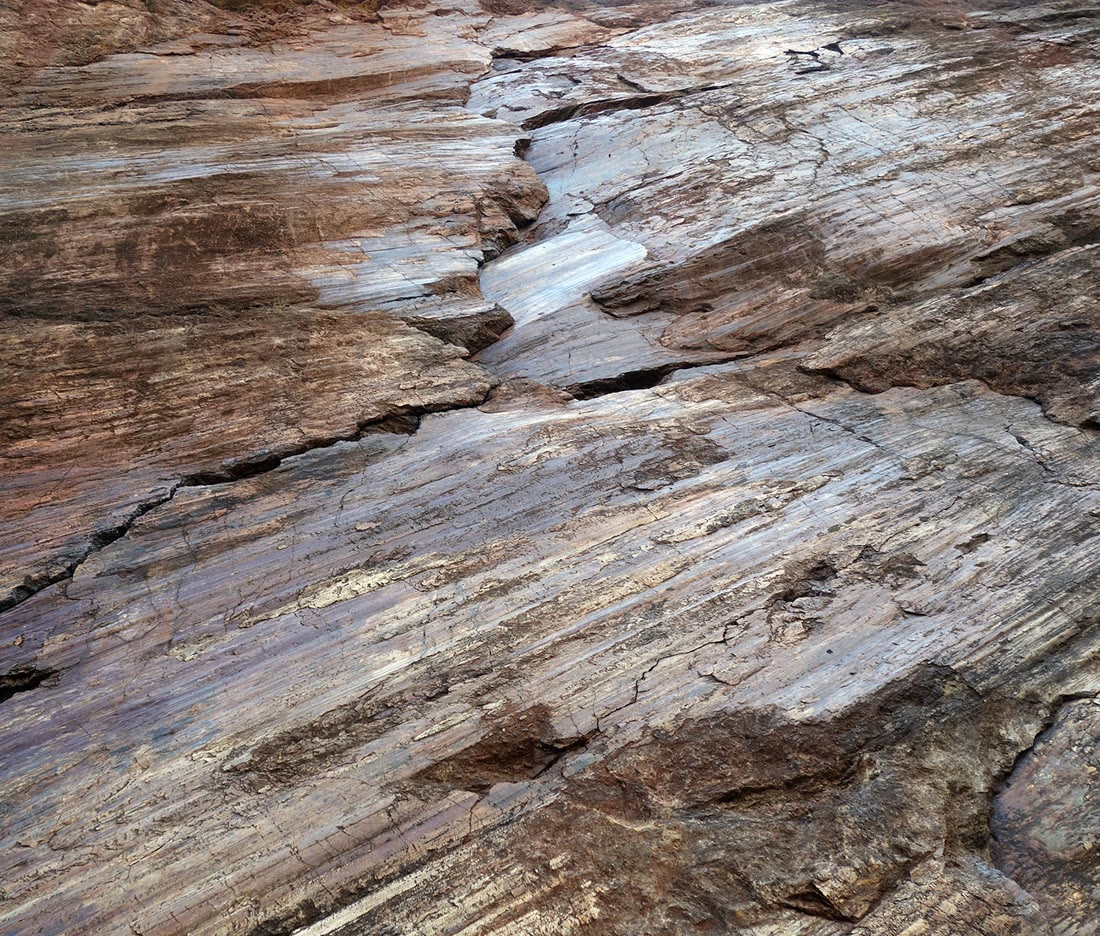
\includegraphics[height=5.2cm]{images/book3/b1-slickenside.jpg}\hfill
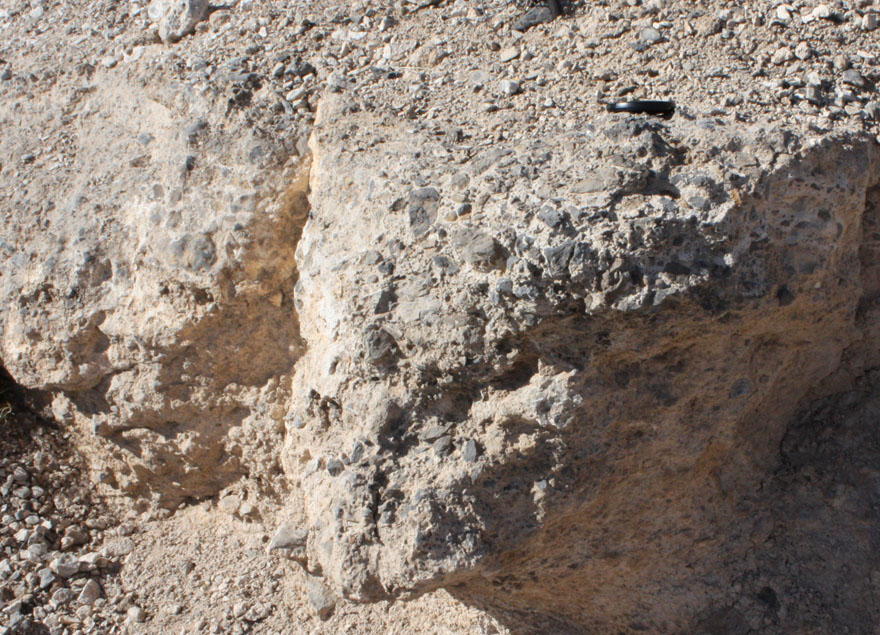
\includegraphics[height=5.2cm]{images/book3/b1-fault-breccia.jpg}
\par\smallskip{\small 左：燧石中断层面上的\omterm{def:b1:faults-folds-fabrics:fault-rocks}{断层镜面}，约
\qtyproduct{3 x 3}{m}见方的面（高 \qty{10}{m}），位于旧金山科罗纳高地；
抛光面沿滑动方向具条纹。照片：
Dextersinister, CC~BY-SA~4.0。右：内华达州红岩峡谷基斯顿\omterm{def:b1:faults-folds-fabrics:fault-types}{逆冲断层}的
\omterm{def:b1:faults-folds-fabrics:fault-rocks}{断层角砾岩}：棱角状的灰色碳酸盐岩碎块，嵌于较浅色的
基质中；右上角镜头盖直径为 \qty{5.8}{cm}。照片：
Jstuby，公有领域。两图均来自维基共享资源。}
\label{fig:b1:faults-folds-fabrics:fault-surfaces}
\end{omfigure}
% ledger: commons:slickenside, commons:breccia

\begin{method}[测量断层的滑距]\label{met:b1:faults-folds-fabrics:slip}
\begin{enumerate}
  \item 测量断层面的\omterm{def:b1:geological-maps:attitude}{产状} $\alpha/\delta$，
        并写出其\omterm{def:b1:geological-maps:attitude}{走向} $\alpha - \ang{90}$。
  \item 测量\omterm{def:b1:faults-folds-fabrics:fault-rocks}{擦痕}：其在断层上的\omterm{def:b1:faults-folds-fabrics:fault-elements}{侧伏角}，或其\omterm{def:b1:field-lab-methods-1:trend-plunge}{倾伏向}
        与\omterm{def:b1:field-lab-methods-1:trend-plunge}{倾伏角}；对\omterm{def:b1:faults-folds-fabrics:fault-elements}{侧伏角} $r$，有 $\sin p = |\sin r|\sin\delta$。
  \item 由断层两侧错开的标志，判断\omterm{def:b1:faults-folds-fabrics:fault-elements}{上盘}的运动方向，
        并为\omterm{def:b1:faults-folds-fabrics:fault-elements}{侧伏角}定号：
        \omterm{def:b1:faults-folds-fabrics:fault-elements}{上盘}下降时取负号。
  \item 由原为一点的两点求出\omterm{def:b1:faults-folds-fabrics:fault-elements}{总滑距} $L$；若只知水平标志层的
        \omterm{def:b1:cross-sections:throw}{垂直断距} $h$，则 $L = h/(|\sin r|\sin\delta)$。
  \item 用\cref{prop:b1:faults-folds-fabrics:slip-components}计算各分量，
        并依据
        \cref{def:b1:faults-folds-fabrics:fault-types}为断层命名。
\end{enumerate}
\end{method}

\begin{inthefield}[测量断层面]
地质学家在\omterm{def:b1:geological-maps:geological-map}{露头}中发现断层面后，与测量其他平面一样，
将罗盘–测斜仪贴于断层面上测其\omterm{def:b1:geological-maps:attitude}{产状}，再测量其上的\omterm{def:b1:faults-folds-fabrics:fault-rocks}{擦痕}，
\omterm{def:b1:faults-folds-fabrics:fault-rocks}{擦痕}可以\omterm{def:b1:faults-folds-fabrics:fault-elements}{侧伏角}表示（以量角器贴于平面上测量），或
以\omterm{def:b1:field-lab-methods-1:trend-plunge}{倾伏向}和\omterm{def:b1:field-lab-methods-1:trend-plunge}{倾伏角}表示。两者须借助上述方法第 2 步的公式
相互核对。运动方向的判断最为困难。断层面上的小阶步，
以及块体分离时生长的石英或方解石纤维，
可以指示缺失块体的运动方向，但有些阶步指向相反，
因此只有与标志层或脉体的错断相符时，才采信运动方向。
\omterm{def:b1:faults-folds-fabrics:fault-rocks}{断层岩}需描述并采样；无法在一处测量的宽大断层带，
则在图上填绘为一个带。每条断层都记入笔记本的编号测站，
并记下其\omterm{def:b1:geological-maps:attitude}{产状}、
\omterm{def:b1:faults-folds-fabrics:fault-rocks}{擦痕}、运动方向，以及地质学家对其的把握程度。
\end{inthefield}

\section{安德森断层理论}\label{sec:b1:faults-folds-fabrics:anderson}

为什么多数\omterm{def:b1:faults-folds-fabrics:fault-types}{正断层}较陡，多数\omterm{def:b1:faults-folds-fabrics:fault-types}{逆冲断层}较缓？1905 年，苏格兰
地质学家欧内斯特·马森·安德森以两点论断作答：地球表面决定了
\omterm{def:b1:stress-strain-rheology:principal}{主应力}的方向，随后库仑判据
决定了断层的\omterm{def:b1:geological-maps:attitude}{倾角}。
% ledger: ws:anderson, anderson:1905

\begin{proposition}[自由表面构成一个主平面]\label{prop:b1:faults-folds-fabrics:free-surface}
在水平的地球表面，一个\omterm{def:b1:stress-strain-rheology:principal}{主应力}
竖直，另外两个\omterm{def:b1:stress-strain-rheology:principal}{主应力}水平。
\end{proposition}

\begin{proof}
空气仅以垂直于表面的压强作用于地面：
它不产生切应力。因此，地表水平面上的应力
垂直于该平面。三维情形下，单位法向量为
$\mathbf n$ 的平面上的应力为矢量 $\boldsymbol\sigma\mathbf n$（见本科三年级物理学教材）；
若其无切向分量，则它与 $\mathbf n$ 平行，于是
$\boldsymbol\sigma\mathbf n = \lambda\mathbf n$，故 $\mathbf n$ 是对称矩阵 $\boldsymbol\sigma$ 的
特征向量，即
一个主方向（见\cref{def:b1:stress-strain-rheology:principal}）。于是竖直方向是一个主方向，
而与之垂直的另外两个方向
为水平方向。
\end{proof}

安德森假定，\omterm{def:b1:stress-strain-rheology:principal}{主应力}的这些方向一直保持
到断层形成的深度。此假定在地表平缓倾斜、
且岩石中无强烈旧弱面的情形下较为可靠；在陡峭地形附近，
以及旧断层或岩层引导新断层的地方，则不成立。在此假定下，
根据 $\sigma_1$、$\sigma_2$ 与
$\sigma_3$ 中哪一个竖直，只有三种情形可能。

\begin{theorem}[安德森断层理论]\label{thm:b1:faults-folds-fabrics:anderson}
设一个\omterm{def:b1:stress-strain-rheology:principal}{主应力}竖直，岩石按库仑判据破裂，
\omterm{def:b1:stress-strain-rheology:coulomb}{内摩擦角}为 $\phi$。新断层形成于包含 $\sigma_2$ 方向的面上，
这些面的夹角为 $\ang{45} - \phi/2$，即与 $\sigma_1$ 所成的角，
并沿垂直于 $\sigma_2$ 的方向滑动，
沿 $\sigma_1$ 方向缩短岩石。由此
\begin{enumerate}[label=(\alph*)]
  \item 若 $\sigma_1$ 竖直，则形成\omterm{def:b1:faults-folds-fabrics:fault-types}{正断层}，\omterm{def:b1:geological-maps:attitude}{走向}沿
        $\sigma_2$ 方向，\omterm{def:b1:geological-maps:attitude}{倾角}为 $\ang{45} + \phi/2$；
  \item 若 $\sigma_3$ 竖直，则形成\omterm{def:b1:faults-folds-fabrics:fault-types}{逆冲断层}，\omterm{def:b1:geological-maps:attitude}{走向}沿
        $\sigma_2$ 方向，\omterm{def:b1:geological-maps:attitude}{倾角}为 $\ang{45} - \phi/2$；
  \item 若 $\sigma_2$ 竖直，则形成竖直的\omterm{def:b1:faults-folds-fabrics:fault-types}{走滑断层}，\omterm{def:b1:geological-maps:attitude}{走向}
        为 $\ang{45} - \phi/2$，分列于 $\sigma_1$ 两侧。
\end{enumerate}
取 $\phi = \ang{30}$ 时，三种情形的\omterm{def:b1:geological-maps:attitude}{倾角}分别为 \ang{60}、\ang{30} 和 \ang{90}。
\end{theorem}
\index{安德森断层理论}

\begin{proof}
若平面包含 $\sigma_2$ 方向，则其法向位于
$\sigma_1$ 与 $\sigma_3$ 所在的平面内，该平面上的应力即为
即\cref{ch:b1:stress-strain-rheology}中的二维问题：其点
位于 $\sigma_1$ 与 $\sigma_3$ 的莫尔圆上，其切向部分位于
$\sigma_1$ 与 $\sigma_3$ 所在的平面内，且垂直于 $\sigma_2$。在其他任何
平面上，点 $(\sigma_n, \tau)$ 位于该圆之内，而该圆是
三维应力状态三个莫尔圆中最大的一个
（由三维理论在本阶段不加证明地承认）。随着应力增大，库仑
线因此首先与包含 $\sigma_2$ 的平面相切，而在其中，
由\cref{thm:b1:stress-strain-rheology:failure-angle}可知，相切的是
夹角为 $\ang{45} - \phi/2$、以 $\sigma_1$ 为基准的那些平面。
沿此类平面的滑动，方向垂直于 $\sigma_2$，使两块体沿最大压缩方向相互靠近，
沿最小压缩方向相互分离，以释放应力。情形 (a) 中，
该平面与竖直方向的夹角为 $\ang{45} - \phi/2$，
故其\omterm{def:b1:geological-maps:attitude}{倾角}为 $\ang{45} + \phi/2$，\omterm{def:b1:geological-maps:attitude}{走向}沿水平的 $\sigma_2$ 方向；
滑动位于\omterm{def:b1:geological-maps:attitude}{倾向}所在的竖直面内，\omterm{def:b1:faults-folds-fabrics:fault-elements}{上盘}下降，
使岩石水平伸长：\omterm{def:b1:faults-folds-fabrics:fault-types}{正断层}。情形 (b) 中，
该平面与水平方向的夹角为 $\ang{45} - \phi/2 < \ang{45}$，水平方向即 $\sigma_1$，
滑动使岩石水平缩短，\omterm{def:b1:faults-folds-fabrics:fault-elements}{上盘}被推起：\omterm{def:b1:faults-folds-fabrics:fault-types}{逆冲断层}。情形 (c) 中，
平面包含竖直方向，故为竖直面；滑动水平，
且垂直于 $\sigma_2$：\omterm{def:b1:faults-folds-fabrics:fault-types}{走滑断层}，
\omterm{def:b1:geological-maps:attitude}{走向}各偏转 $\ang{45} - \phi/2$，分列于水平的 $\sigma_1$ 两侧。
\end{proof}

每种情形下都可能出现两组关于 $\sigma_1$ 对称的断层：
共轭断层，相交于 $\ang{90} - \phi$（约 \ang{60}），
$\sigma_1$ 位于二者所夹的锐角之中。反之，野外实测的一对共轭
断层可给出形成它们的应力方向：
$\sigma_1$ 平分其锐角，$\sigma_2$ 为
二者的交线。

\begin{omfigure}
\begin{tikzpicture}[x={(1cm,0cm)}, y={(0.42cm,0.30cm)}, z={(0cm,1cm)},
  >={Stealth[length=5pt]}, font=\small, scale=0.86,
  face/.style={draw=black, line width=0.5pt, line join=round},
  sone/.style={->, line width=1.6pt, omThm},
  sthree/.style={->, line width=0.8pt, omDef}]
% exact geometry: the fault plane is X = xf(Z); slip is along the dip; throw t
% (a) normal fault: dip 60, xf(Z) = 1.3 + (1.6 - Z)/tan 60, throw 0.45
\begin{scope}
  \def\W{3.2}\def\D{1.6}\def\H{1.6}
  \pgfmathsetmacro{\c}{1/tan(60)}
  \pgfmathsetmacro{\xa}{1.3+1.6*\c}       % xf(0)
  \pgfmathsetmacro{\xb}{1.3+0.45*\c}      % xf(H - t)
  \pgfmathsetmacro{\mfa}{1.3+(1.6-0.55)*\c}\pgfmathsetmacro{\mfb}{1.3+(1.6-0.85)*\c}
  \pgfmathsetmacro{\mha}{1.3+(1.6-0.10)*\c}\pgfmathsetmacro{\mhb}{1.3+(1.6-0.40)*\c}
  % footwall
  \fill[omLithSand!55] (0,0,0) -- (\xa,0,0) -- (1.3,0,\H) -- (0,0,\H) -- cycle;
  \fill[omProp!40] (0,0,0.55) -- (\mfa,0,0.55) -- (\mfb,0,0.85) -- (0,0,0.85) -- cycle;
  \draw[face] (0,0,0) -- (\xa,0,0) -- (1.3,0,\H) -- (0,0,\H) -- cycle;
  \draw[face, fill=omLithSand!35] (0,0,\H) -- (1.3,0,\H) -- (1.3,\D,\H) -- (0,\D,\H) -- cycle;
  \draw[face, fill=black!12] (1.3,0,\H) -- (\xb,0,1.15) -- (\xb,\D,1.15) -- (1.3,\D,\H) -- cycle;
  % hanging wall
  \fill[omLithSand!55] (\xa,0,0) -- (\W,0,0) -- (\W,0,1.15) -- (\xb,0,1.15) -- cycle;
  \fill[omProp!40] (\mha,0,0.10) -- (\W,0,0.10) -- (\W,0,0.40) -- (\mhb,0,0.40) -- cycle;
  \draw[face] (\xa,0,0) -- (\W,0,0) -- (\W,0,1.15) -- (\xb,0,1.15) -- cycle;
  \draw[face, fill=omLithSand!35] (\xb,0,1.15) -- (\W,0,1.15) -- (\W,\D,1.15) -- (\xb,\D,1.15) -- cycle;
  \fill[omLithSand!45] (\W,0,0) -- (\W,\D,0) -- (\W,\D,1.15) -- (\W,0,1.15) -- cycle;
  \fill[omProp!30] (\W,0,0.10) -- (\W,\D,0.10) -- (\W,\D,0.40) -- (\W,0,0.40) -- cycle;
  \draw[face] (\W,0,0) -- (\W,\D,0) -- (\W,\D,1.15) -- (\W,0,1.15) -- cycle;
  % slip arrow on the front face
  \draw[->, line width=0.9pt] (1.45,0,1.05) -- ++({0.35*cos(60)},0,{-0.35*sin(60)});
  % stresses: sigma1 vertical, sigma3 horizontal across the strike
  \draw[sone] (1.6,0.8,3.05) -- (1.6,0.8,2.1) node[pos=0, left] {$\sigma_1$};
  \draw[sone] (1.6,0.8,-1.1) -- (1.6,0.8,-0.15);
  \draw[sthree] (-0.85,0.8,0.8) -- (-0.15,0.8,0.8) node[pos=0, above] {$\sigma_3$};
  \draw[sthree] (4.05,0.8,0.6) -- (3.35,0.8,0.6);
  \node[font=\small\bfseries] at (1.9,0,-1.55) {(a) 正断层};
\end{scope}
% (b) thrust fault: dip 30, xf(Z) = 3.0 - Z/tan 30, throw 0.35, heave 0.606
\begin{scope}[xshift=6.0cm]
  \def\D{1.6}\def\H{1.3}
  \pgfmathsetmacro{\c}{1/tan(30)}
  \pgfmathsetmacro{\Wp}{4.0-0.35*\c}       % right face of the hanging wall
  \pgfmathsetmacro{\xt}{3.0-1.3*\c}        % footwall top edge
  \pgfmathsetmacro{\xh}{3.0-1.65*\c}       % hanging-wall top edge
  \pgfmathsetmacro{\mfa}{3.0-0.50*\c}\pgfmathsetmacro{\mfb}{3.0-0.75*\c}
  \pgfmathsetmacro{\mha}{3.0-0.85*\c}\pgfmathsetmacro{\mhb}{3.0-1.10*\c}
  % footwall
  \fill[omLithSand!55] (0,0,0) -- (3.0,0,0) -- (\xt,0,\H) -- (0,0,\H) -- cycle;
  \fill[omProp!40] (0,0,0.50) -- (\mfa,0,0.50) -- (\mfb,0,0.75) -- (0,0,0.75) -- cycle;
  \draw[face] (0,0,0) -- (3.0,0,0) -- (\xt,0,\H) -- (0,0,\H) -- cycle;
  \draw[face, fill=omLithSand!35] (0,0,\H) -- (\xt,0,\H) -- (\xt,\D,\H) -- (0,\D,\H) -- cycle;
  % hanging wall
  \fill[omLithSand!55] (3.0,0,0) -- (\Wp,0,0) -- (\Wp,0,1.65) -- (\xh,0,1.65) -- cycle;
  \fill[omProp!40] (\mha,0,0.85) -- (\Wp,0,0.85) -- (\Wp,0,1.10) -- (\mhb,0,1.10) -- cycle;
  \draw[face] (3.0,0,0) -- (\Wp,0,0) -- (\Wp,0,1.65) -- (\xh,0,1.65) -- cycle;
  \draw[face, fill=omLithSand!35] (\xh,0,1.65) -- (\Wp,0,1.65) -- (\Wp,\D,1.65) -- (\xh,\D,1.65) -- cycle;
  \fill[omLithSand!45] (\Wp,0,0) -- (\Wp,\D,0) -- (\Wp,\D,1.65) -- (\Wp,0,1.65) -- cycle;
  \fill[omProp!30] (\Wp,0,0.85) -- (\Wp,\D,0.85) -- (\Wp,\D,1.10) -- (\Wp,0,1.10) -- cycle;
  \draw[face] (\Wp,0,0) -- (\Wp,\D,0) -- (\Wp,\D,1.65) -- (\Wp,0,1.65) -- cycle;
  \draw[->, line width=0.9pt] (2.25,0,0.62) -- ++({-0.42*cos(30)},0,{0.42*sin(30)});
  % stresses: sigma1 horizontal across the strike, sigma3 vertical
  \draw[sone] (-1.2,0.8,0.65) -- (-0.15,0.8,0.65) node[pos=0, above] {$\sigma_1$};
  \draw[sone] (\Wp+1.15,0.8,0.45) -- (\Wp+0.1,0.8,0.45);
  \draw[sthree] (2.0,0.8,2.7) -- (2.0,0.8,2.0) node[pos=0, left] {$\sigma_3$};
  \draw[sthree] (2.0,0.8,-0.9) -- (2.0,0.8,-0.2);
  \node[font=\small\bfseries] at (2.0,0,-1.55) {(b) 逆冲断层};
\end{scope}
% (c) strike-slip fault: vertical, along the y axis at X = 1.6; dextral: the far
% (east) block has moved toward the reader by 0.5; sigma1 at 30 deg clockwise of the strike
\begin{scope}[xshift=12.0cm]
  \def\D{2.2}\def\H{1.1}\def\s{0.5}
  % west block
  \draw[face, fill=omLithSand!55] (0,0,0) -- (1.6,0,0) -- (1.6,0,\H) -- (0,0,\H) -- cycle;
  \draw[face, fill=omLithSand!35] (0,0,\H) -- (1.6,0,\H) -- (1.6,\D,\H) -- (0,\D,\H) -- cycle;
  \draw[face, fill=black!12] (1.6,\D-\s,0) -- (1.6,\D,0) -- (1.6,\D,\H) -- (1.6,\D-\s,\H) -- cycle;
  \draw[line width=1.4pt, omProp] (0,1.25,\H) -- (1.6,1.25,\H);
  % east block
  \draw[face, fill=omLithSand!55] (1.6,-\s,0) -- (3.2,-\s,0) -- (3.2,-\s,\H) -- (1.6,-\s,\H) -- cycle;
  \draw[face, fill=omLithSand!35] (1.6,-\s,\H) -- (3.2,-\s,\H) -- (3.2,\D-\s,\H) -- (1.6,\D-\s,\H) -- cycle;
  \draw[face, fill=omLithSand!45] (3.2,-\s,0) -- (3.2,\D-\s,0) -- (3.2,\D-\s,\H) -- (3.2,-\s,\H) -- cycle;
  \draw[line width=1.4pt, omProp] (1.6,1.25-\s,\H) -- (3.2,1.25-\s,\H);
  % slip arrows on the top
  \draw[->, line width=0.9pt] (2.05,1.35,\H) -- (2.05,0.35,\H);
  \draw[->, line width=0.9pt] (1.15,0.55,\H) -- (1.15,1.55,\H);
  % stresses in the horizontal plane, drawn at the height of the top surface
  \draw[sone] ({1.6+1.9*sin(30)},{0.8+1.9*cos(30)},\H) -- ({1.6+1.0*sin(30)},{0.8+1.0*cos(30)},\H) node[pos=0, right] {$\sigma_1$};
  \draw[sone] ({1.6-1.9*sin(30)},{0.8-1.9*cos(30)},\H) -- ({1.6-1.0*sin(30)},{0.8-1.0*cos(30)},\H);
  \draw[sthree] ({1.6+2.0*sin(120)},{0.8+2.0*cos(120)},\H) -- ({1.6+1.45*sin(120)},{0.8+1.45*cos(120)},\H) node[pos=0, right] {$\sigma_3$};
  \draw[sthree] ({1.6-2.0*sin(120)},{0.8-2.0*cos(120)},\H) -- ({1.6-1.45*sin(120)},{0.8-1.45*cos(120)},\H);
  \node[font=\small\bfseries] at (1.7,0,-1.55) {(c) 走滑断层};
\end{scope}
\end{tikzpicture}
\par\smallskip{\small 安德森三种应力状态，断层\omterm{def:b1:geological-maps:attitude}{倾角}分别取定理中 $\phi = \ang{30}$ 对应的值：
\ang{60}、\ang{30} 与竖直。粗红箭头为 $\sigma_1$；
细蓝箭头为 $\sigma_3$；$\sigma_2$ 在 (a)、(b) 中沿断层\omterm{def:b1:geological-maps:attitude}{走向}，在 (c) 中竖直。标志层
（橙色）在 (a)、(b) 中被\omterm{def:b1:cross-sections:throw}{垂直断距}错开；在 (c) 中，地面上的一条线
被水平错开，断层为\omterm{def:b1:faults-folds-fabrics:fault-types}{右行}：从任一块体看，
另一块向右移动。
黑色箭头表示滑动方向。}
\label{fig:b1:faults-folds-fabrics:anderson}
\end{omfigure}

三种应力状态与
\cref{ch:b1:rifts-ridges-margins,ch:b1:active-margins}中的三类板块边界相对应。
\omterm{def:b1:layered-earth:lithosphere}{岩石圈}被拉伸时（裂谷与洋脊处），水平应力低于
竖直应力，于是形成\omterm{def:b1:faults-folds-fabrics:fault-types}{正断层}；\omterm{def:b1:layered-earth:lithosphere}{岩石圈}被挤压时（汇聚边缘
与造山带中），水平应力超过岩石的重量，
于是形成\omterm{def:b1:faults-folds-fabrics:fault-types}{逆冲断层}；沿\omterm{def:b1:rifts-ridges-margins:transform}{转换断层}，两个水平应力
夹住竖直应力。\omterm{def:b1:geological-maps:attitude}{倾角}与观测大体相符：
裂谷的\omterm{def:b1:faults-folds-fabrics:fault-types}{正断层}在近地表处\omterm{def:b1:geological-maps:attitude}{倾角}约为 \ang{60}，\omterm{def:b1:faults-folds-fabrics:fault-types}{逆冲断层}
则为低角度\omterm{def:b1:faults-folds-fabrics:fault-types}{逆断层}。例外之处颇具启发：许多\omterm{def:b1:faults-folds-fabrics:fault-types}{正断层}
随深度变缓，某些裂谷剖面显示它们延伸至
近乎水平的剪切带：这些低角度\omterm{def:b1:faults-folds-fabrics:fault-types}{正断层}，即拆离断层，
切穿\omterm{def:b1:layered-earth:layers}{地壳}时\omterm{def:b1:geological-maps:attitude}{倾角}远小于 \ang{45}。安德森理论无法将其
解释为新生断层；由\cref{exo:b1:faults-folds-fabrics:10}可知，
同样地，按\omterm{prop:b1:stress-strain-rheology:byerlee}{拜尔利定律}的摩擦力，它们在安德森应力下也无法滑动：
它们需要弱\omterm{def:b1:faults-folds-fabrics:fault-rocks}{断层岩}、高孔隙压力或旋转的应力。已有断层
按\omterm{prop:b1:stress-strain-rheology:byerlee}{拜尔利定律}的摩擦力滑动，
$\mu = 0.85$，$\phi = \ang{40.4}$；取向最佳的\omterm{def:b1:faults-folds-fabrics:fault-types}{正断层}此时\omterm{def:b1:geological-maps:attitude}{倾角}为
\ang{65.2}，与\cref{ch:b1:stress-strain-rheology}中所求得的结果相符。
% ledger: ws:anderson, usgs:fault-types, byerlee:1975

\begin{history}[安德森的断层]
苏格兰地质学家欧内斯特·马森·安德森于 1905 年发表了关于三类断层的理论，
该理论载于一篇讨论断层动力学的短文，
并在其著作中给出完整形式，并将其用于英国的岩墙与断层，书名为
\emph{The Dynamics of Faulting and Dyke Formation}。少数论文与该书
至今仍塑造着构造地质学、地震学与岩石力学。他提出的三种应力体制，
即\omterm{def:b1:faults-folds-fabrics:fault-types}{正断层}、逆冲与走滑，
是划分\omterm{def:b1:layered-earth:layers}{地壳}应力状态及其所形成断层的常用方式，
也是由断层读取应力的常用方式。
\end{history}
% ledger: anderson:1905, healy:anderson, ws:anderson

\section{褶皱几何}\label{sec:b1:faults-folds-fabrics:folds}

\Cref{ch:b1:geological-maps}中已为\omterm{def:b1:geological-maps:fold}{褶皱}命名，并在地图上读取了它们的形态。
在三维空间中，描述\omterm{def:b1:geological-maps:fold}{褶皱}还需要更多名称：它在何处弯曲、弯曲程度如何，
以及它在空间中如何取向。

\begin{definition}[转折端、枢纽、翼、轴面、翼间角、圆柱状褶皱]\label{def:b1:faults-folds-fabrics:fold-elements}
在\omterm{def:b1:geological-maps:fold}{褶皱}面上，\emph{转折端}\index{转折端}是曲率最大的区域，
\emph{枢纽}\index{枢纽}是连接各曲率最大点的直线；
\emph{翼}\index{翼}是两侧曲率较小的部分。\omterm{def:b1:geological-maps:fold}{褶皱}的
轴面是连接其各相继\omterm{def:b1:geological-maps:fold}{褶皱}面枢纽线的面；
当它为平面时，即为
\emph{轴面}\index{轴面}。
\emph{翼间角}\index{翼间角} $\iota$ 是两翼之间的夹角，在剖面
（与枢纽线垂直的平面）上量取，
为两翼拐点处切线之间的夹角；
$0 \le \iota \le \ang{180}$。若\omterm{def:b1:geological-maps:fold}{褶皱}的各面由一条直线平行于自身移动生成，则称该\omterm{def:b1:geological-maps:fold}{褶皱}为\emph{圆柱状
褶皱}\index{圆柱状褶皱}。该直线的方向即为\omterm{def:b1:geological-maps:fold}{褶皱轴}
（见
\cref{def:b1:geological-maps:fold}），圆柱状\omterm{def:b1:geological-maps:fold}{褶皱}的每条枢纽线
都是平行于该轴的直线。
\end{definition}
% ledger: ws:fold-elements

\begin{omfigure}
\begin{tikzpicture}[x={(1cm,0cm)}, y={(0.42cm,0.30cm)}, z={(0cm,1cm)},
  >={Stealth[length=5pt]}, font=\small, scale=1.15]
% a cylindrical anticline: the top of a bed is z = f(x) = 0.35 a - a sqrt(x^2 + 0.35^2), a = tan 50
% (limbs dip toward 50 deg, interlimb angle 80 deg); the bed is 0.7 thick, measured vertically
% (a similar fold); the fold axis is the y direction, horizontal.
\def\D{2.8}
\pgfmathsetmacro{\a}{tan(50)}
\def\f(#1){0.35*\a - \a*sqrt((#1)*(#1) + 0.1225)}
\pgfmathsetmacro{\zt}{0.35*\a}
% top surface of the bed
\fill[omLithSand!35] plot[domain=-1.7:1.7, samples=61, variable=\x] (\x, 0, {\f(\x)})
  -- plot[domain=1.7:-1.7, samples=61, variable=\x] (\x, \D, {\f(\x)}) -- cycle;
\foreach \u in {-1.4,-1.0,-0.6,-0.3,0.3,0.6,1.0,1.4} {
  \draw[black!35, line width=0.3pt] (\u, 0, {\f(\u)}) -- (\u, \D, {\f(\u)});
}
\draw[line width=0.5pt] plot[domain=-1.7:1.7, samples=61, variable=\x] (\x, \D, {\f(\x)});
\draw[line width=0.5pt] (-1.7, 0, {\f(-1.7)}) -- (-1.7, \D, {\f(-1.7)});
% right end face
\fill[omLithSand!55] (1.7, 0, {\f(1.7)}) -- (1.7, \D, {\f(1.7)}) -- (1.7, \D, {\f(1.7)-0.7}) -- (1.7, 0, {\f(1.7)-0.7}) -- cycle;
\draw[line width=0.5pt] (1.7, 0, {\f(1.7)}) -- (1.7, \D, {\f(1.7)}) -- (1.7, \D, {\f(1.7)-0.7}) -- (1.7, 0, {\f(1.7)-0.7});
% axial plane, behind the front face
\fill[omDef!30, opacity=0.5] (0, 0, 0.85) -- (0, \D, 0.85) -- (0, \D, -2.0) -- (0, 0, -2.0) -- cycle;
\draw[omDef, line width=0.6pt] (0, 0, -2.0) -- (0, 0, 0.85) -- (0, \D, 0.85) -- (0, \D, -2.0);
% hinge line
\draw[omThm, line width=1.5pt] (0, 0, 0) -- (0, \D, 0);
% front face of the bed (the profile)
\fill[omLithSand!80] plot[domain=-1.7:1.7, samples=61, variable=\x] (\x, 0, {\f(\x)})
  -- plot[domain=1.7:-1.7, samples=61, variable=\x] (\x, 0, {\f(\x)-0.7}) -- cycle;
\draw[line width=0.7pt] plot[domain=-1.7:1.7, samples=61, variable=\x] (\x, 0, {\f(\x)});
\draw[line width=0.7pt] plot[domain=-1.7:1.7, samples=61, variable=\x] (\x, 0, {\f(\x)-0.7});
\draw[line width=0.5pt] (-1.7, 0, {\f(-1.7)}) -- (-1.7, 0, {\f(-1.7)-0.7});
\draw[omDef, line width=0.6pt, dashed] (0, 0, 0) -- (0, 0, -0.7);
\draw[omDef, line width=0.6pt] (0, 0, -0.7) -- (0, 0, -2.0);
% interlimb angle on the profile, in the core: tangents to the limbs of the base of the bed
% meet at (0, 0, zt - 0.7)
\pgfmathsetmacro{\zb}{\zt-0.7}
\draw[black!70, dashed] (-1.3, 0, {\zb-1.3*\a}) -- (0, 0, \zb) -- (1.3, 0, {\zb-1.3*\a});
\draw[black, line width=0.5pt] plot[domain=-140:-40, samples=21, variable=\t] ({0.75*cos(\t)}, 0, {\zb+0.75*sin(\t)});
\node[font=\scriptsize] at (0.22, 0, {\zb-1.0}) {$\iota$};
% labels
\node[omThm, anchor=west, font=\scriptsize] at (0.08, \D, 0.1) {枢纽};
\node[omDef, anchor=south, font=\scriptsize] at (0, \D, 0.85) {轴面};
\node[font=\scriptsize, rotate=50] at (-1.15, 0, {\f(-1.15)-0.35}) {翼};
\node[font=\scriptsize, rotate=-50] at (1.15, 0, {\f(1.15)-0.35}) {翼};
\end{tikzpicture}
\par\smallskip{\small 圆柱状\omterm{def:b1:geological-maps:fold}{背斜}的各要素，此处\omterm{def:b1:faults-folds-fabrics:fold-elements}{枢纽}线水平：\omterm{def:b1:faults-folds-fabrics:fold-elements}{转折端}，即岩层弯曲最剧烈处；两翼；
穿过岩层顶面与底面\omterm{def:b1:faults-folds-fabrics:fold-elements}{枢纽}线的\omterm{def:b1:faults-folds-fabrics:fold-elements}{轴面}；
以及两翼切线之间的\omterm{def:b1:faults-folds-fabrics:fold-elements}{翼间角} $\iota$，
在剖面前缘处量取，此处为\ang{80}，
画于岩层底面。岩层顶面上的灰线
与\omterm{def:b1:geological-maps:fold}{褶皱轴}平行。}
\label{fig:b1:faults-folds-fabrics:fold-elements}
\end{omfigure}

当两翼为平面时，如下文的人字\omterm{def:b1:geological-maps:fold}{褶皱}及
瓦尔登丘陵中的情形，\omterm{def:b1:geological-maps:fold}{褶皱}的几何形态可由其两翼的\omterm{def:b1:geological-maps:attitude}{产状}确定。
\omterm{def:b1:geological-maps:attitude}{倾向}为 $\alpha$、\omterm{def:b1:geological-maps:attitude}{倾角}为 $\delta$ 的平面的向上单位法向量为
$\mathbf n = (\sin\delta\sin\alpha, \sin\delta\cos\alpha, \cos\delta)$，其分量依次为
东、北、上三个方向的分量。

\begin{proposition}[由两翼确定褶皱]\label{prop:b1:faults-folds-fabrics:hinge}
设\omterm{def:b1:faults-folds-fabrics:fold-elements}{圆柱状褶皱}的两翼均为平面且均未倒转，其向上的单位法向量
分别为 $\mathbf n_1$ 与 $\mathbf n_2$。其\omterm{def:b1:faults-folds-fabrics:fold-elements}{枢纽}线平行于
$\mathbf n_1 \times \mathbf n_2$，其\omterm{def:b1:faults-folds-fabrics:fold-elements}{翼间角}为
\[
  \iota = \ang{180} - \arccos(\mathbf n_1\cdot\mathbf n_2) .
\]
\end{proposition}

\begin{proof}
每个翼由平行于\omterm{def:b1:geological-maps:fold}{褶皱轴}的直线生成，因此包含该轴的方向，
该轴方向与两法向量都垂直，
从而平行于它们的叉积；\omterm{def:b1:faults-folds-fabrics:fold-elements}{枢纽}线与该轴平行。
剖面与\omterm{def:b1:geological-maps:fold}{褶皱轴}垂直，因此包含两个法向量；在剖面中，两翼表现为两条直线，
分别与 $\mathbf n_1$ 和
$\mathbf n_2$ 垂直，两直线之间的夹角等于
$\arccos(\mathbf n_1\cdot\mathbf n_2)$，即两法向量之间的夹角或其补角。
岩层未\omterm{def:b1:geological-maps:fold}{褶皱}时，两法向量重合，\omterm{def:b1:faults-folds-fabrics:fold-elements}{翼间角}为
\ang{180}；随着两翼转动，两法向量之间的夹角由
$0$ 开始增大，\omterm{def:b1:faults-folds-fabrics:fold-elements}{翼间角}则由 \ang{180} 减小，使得二者
之和始终为\ang{180}，只要两法向量均指向上方。
\end{proof}

对于\omterm{def:b1:faults-folds-fabrics:fold-classes}{直立褶皱}，若其两翼在两侧的\omterm{def:b1:geological-maps:attitude}{倾角}均为 $\delta$，则两法向量的夹角为
$2\delta$，且 $\iota = \ang{180} - 2\delta$。

\begin{definition}[褶皱的分类]\label{def:b1:faults-folds-fabrics:fold-classes}
按\omterm{def:b1:faults-folds-fabrics:fold-elements}{翼间角}，\omterm{def:b1:geological-maps:fold}{褶皱}可分为\emph{平缓褶皱}\index{平缓褶皱}
（$\iota$ 从 \ang{180} 到 \ang{170}）、\emph{开阔褶皱}\index{开阔褶皱}
（从 \ang{170} 到 \ang{90}）、\emph{紧闭褶皱}\index{紧闭褶皱}（从 \ang{90} 到
\ang{10}）；若两翼近乎平行（$\iota$ 从 \ang{10} 到
$0$），则为\emph{等斜褶皱}\index{等斜褶皱}。按\omterm{def:b1:faults-folds-fabrics:fold-elements}{轴面}\omterm{def:b1:geological-maps:attitude}{倾角}分类，
\omterm{def:b1:geological-maps:attitude}{倾角}大于 \ang{80} 时为\emph{直立褶皱}\index{直立褶皱}，
\omterm{def:b1:geological-maps:attitude}{倾角}小于 \ang{10} 时为\emph{平卧褶皱}\index{平卧褶皱}，
介于两者之间的为\emph{斜歪褶皱}\index{斜歪褶皱}。
若某一翼已转过竖直方向，
使两翼\omterm{def:b1:geological-maps:attitude}{倾向}相同，且该翼的岩层倒置，
则称为\emph{倒转褶皱}\index{倒转褶皱}。
\omterm{def:b1:faults-folds-fabrics:fold-elements}{枢纽}线不水平的\omterm{def:b1:geological-maps:fold}{褶皱}，
称为\emph{倾伏褶皱}\index{倾伏褶皱}。
\end{definition}
对于紧密程度的分类，文献中还使用其他界限；
本书采用上述四类。
% ledger: ws:fold-classes, ws:fold-elements

\begin{omfigure}
\begin{tikzpicture}[font=\small]
% one antiform profile: a hinge arc of radius 0.22 and two straight limbs of length 1.05,
% each at half the interlimb angle (#1 = iota/2) from the downward axial trace; three
% surfaces repeated by a shift of 0.3 along the axial trace (a similar fold)
\newcommand{\foldprof}[2]{%
  \foreach \k in {0,1,2} {
    \draw[line width=0.7pt, #2]
      ($(0,-0.3*\k)+(180-#1:0.22)+({-1.05*sin(#1)},{-1.05*cos(#1)})$)
      -- ($(0,-0.3*\k)+(180-#1:0.22)$)
      arc[start angle=180-#1, end angle=#1, radius=0.22]
      -- ++({1.05*sin(#1)},{-1.05*cos(#1)});
  }
}
% row 1: tightness (the axial plane vertical)
\foreach \i/\n/\x in {174/平缓/1.5, 120/开阔/4.5, 50/紧闭/7.5, 0/等斜/10.5} {
  \begin{scope}[xshift=\x cm]
    \pgfmathsetmacro{\b}{\i/2}
    \draw[omDef, dashed, line width=0.5pt] (0,0.45) -- (0,-1.85);
    \foldprof{\b}{black}
    \node[font=\small\bfseries] at (0,-2.2) {\n};
    \node[font=\scriptsize] at (0,-2.6) {$\iota = \ang{\i}$};
  \end{scope}
}
% row 2: attitude of the axial plane (iota = 40 deg)
\foreach \d/\n/\x in {90/直立/1.5, 50/斜歪/6.0, 8/平卧/10.5} {
  \begin{scope}[xshift=\x cm, yshift=-4.3cm]
    \begin{scope}[rotate={-(90-\d)}]
      \draw[omDef, dashed, line width=0.5pt] (0,0.55) -- (0,-1.85);
      \foldprof{20}{black}
    \end{scope}
    \node[font=\small\bfseries] at (0,-2.2) {\n};
    \node[font=\scriptsize] at (0,-2.6) {轴面倾角 \ang{\d}};
  \end{scope}
}
\end{tikzpicture}
\par\smallskip{\small \omterm{def:b1:geological-maps:fold}{褶皱}剖面示意图。上：按\omterm{def:b1:faults-folds-fabrics:fold-elements}{翼间角}分类，\omterm{def:b1:faults-folds-fabrics:fold-elements}{轴面}竖直（虚线）。
下：按\omterm{def:b1:faults-folds-fabrics:fold-elements}{轴面}\omterm{def:b1:geological-maps:attitude}{倾角}分类，图中\omterm{def:b1:geological-maps:fold}{褶皱}的\omterm{def:b1:faults-folds-fabrics:fold-elements}{翼间角}为 \ang{40}。
所画的\omterm{def:b1:faults-folds-fabrics:fold-classes}{斜歪褶皱}同时也是倒转的，
两翼均向左倾。}
\label{fig:b1:faults-folds-fabrics:classes}
\end{omfigure}

岩层的厚度可区分两种样式。平行\omterm{def:b1:geological-maps:fold}{褶皱}（或称同心\omterm{def:b1:geological-maps:fold}{褶皱}）中，
每一层沿垂直于层面方向测得的厚度保持不变，
正如一叠纸张弯曲时的情形；这类\omterm{def:b1:geological-maps:fold}{褶皱}由夹于
极弱层之间的强层屈曲形成。相似\omterm{def:b1:geological-maps:fold}{褶皱}中，每个面的形状都相同，
岩层沿平行于\omterm{def:b1:faults-folds-fabrics:fold-elements}{轴面}方向测得的厚度保持不变，
两翼变薄、\omterm{def:b1:faults-folds-fabrics:fold-elements}{转折端}变厚，如上图剖面所示；
当所有岩层都很弱、不起力学作用时形成。
尖棱\omterm{def:b1:geological-maps:fold}{褶皱}的两翼近乎平直，\omterm{def:b1:faults-folds-fabrics:fold-elements}{转折端}狭窄，
\omterm{def:b1:faults-folds-fabrics:fold-elements}{翼间角}接近 \ang{60}；它们是紧密排列的强层
形成的平行\omterm{def:b1:geological-maps:fold}{褶皱}，
弯曲时各层彼此滑动。
% ledger: ws:fold-elements

\begin{omfigure}
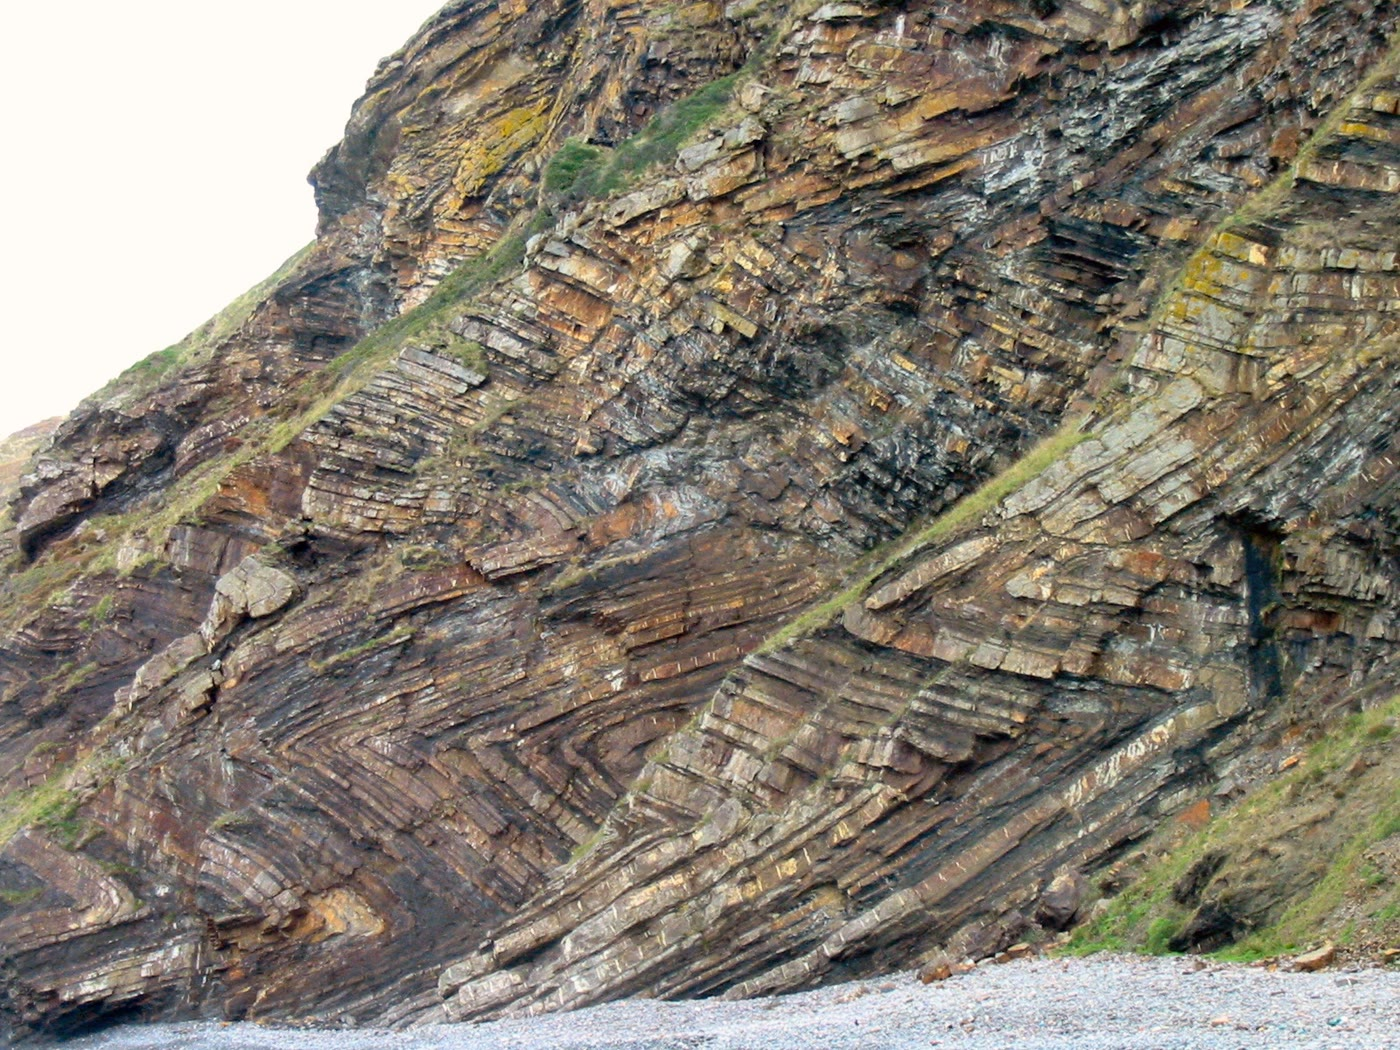
\includegraphics[width=0.78\linewidth]{images/book3/b1-chevron-folds-millook.jpg}
\par\smallskip{\small 北康沃尔米卢克悬崖上\omterm{def:b1:geological-maps:fold}{褶皱}的砂岩与页岩层：尖棱\omterm{def:b1:geological-maps:fold}{褶皱}，
两翼近乎平直，\omterm{def:b1:faults-folds-fabrics:fold-elements}{转折端}尖锐，\omterm{def:b1:faults-folds-fabrics:fold-elements}{轴面}近乎竖直。
照片：Smalljim, CC~BY~3.0
（维基共享资源）。}
\label{fig:b1:faults-folds-fabrics:chevrons}
\end{omfigure}
% ledger: commons:millook

\section{组构}\label{sec:b1:faults-folds-fabrics:fabrics}

变形岩石往往整体变形，而不仅限于少数几个面：其
颗粒被压扁、转动或重新生长为共同方向，从而形成
组构。面状组构使岩石易于劈开，线状组构使岩石易于断裂
成棒状。

\begin{definition}[面理、片理、板劈理、轴面劈理]\label{def:b1:faults-folds-fabrics:foliation}
\emph{面理}\index{面理}是遍及岩石的面状组构：
由一组间距很小的平行面构成，这些面由排列的板状或扁平颗粒
或薄层形成，岩石沿这些面最易劈开。
\emph{片理}\index{片理}是片岩的面理，由排列的
粒径大于约 \qty{1}{mm} 的颗粒形成。\emph{劈理}\index{劈理 （岩石）}
是细粒岩石因变形而形成的面理；
\emph{板劈理}\index{板劈理}是板岩的劈理，由肉眼不可见的
\omterm{def:b1:rock-forming-minerals:silicate-classes}{层状硅酸盐}\omterm{def:b1:rock-forming-minerals:mineral}{矿物}形成，排列十分紧密，
使岩石几乎可在任意位置裂成\omterm{def:b1:field-lab-methods-1:thin-section}{薄片}。
\emph{轴面劈理}\index{轴面劈理}
是与同一岩石中\omterm{def:b1:geological-maps:fold}{褶皱}的\omterm{def:b1:faults-folds-fabrics:fold-elements}{轴面}平行
或近似平行的劈理。
\end{definition}
% ledger: ws:fabrics

\omterm{def:b1:faults-folds-fabrics:foliation}{面理}大致垂直于最大缩短方向形成，
由板状颗粒转动、新\omterm{def:b1:rock-forming-minerals:groups}{云母}生长，以及
受挤压最强的面上颗粒溶解而形成。板岩的\omterm{def:b1:faults-folds-fabrics:foliation}{劈理}
因此与泥的层理毫无关系：它记录的是
挤压作用。当\omterm{def:b1:geological-maps:fold}{褶皱}与\omterm{def:b1:faults-folds-fabrics:foliation}{劈理}在同一缩短过程中形成时，\omterm{def:b1:faults-folds-fabrics:foliation}{劈理}
靠近\omterm{def:b1:geological-maps:fold}{褶皱}的\omterm{def:b1:faults-folds-fabrics:fold-elements}{轴面}，并在\omterm{def:b1:faults-folds-fabrics:fold-elements}{轴面}两侧略呈扇形展开，
各层因强度不同而会聚或发散，
如下图所示。
% ledger: ws:fabrics

\begin{omfigure}
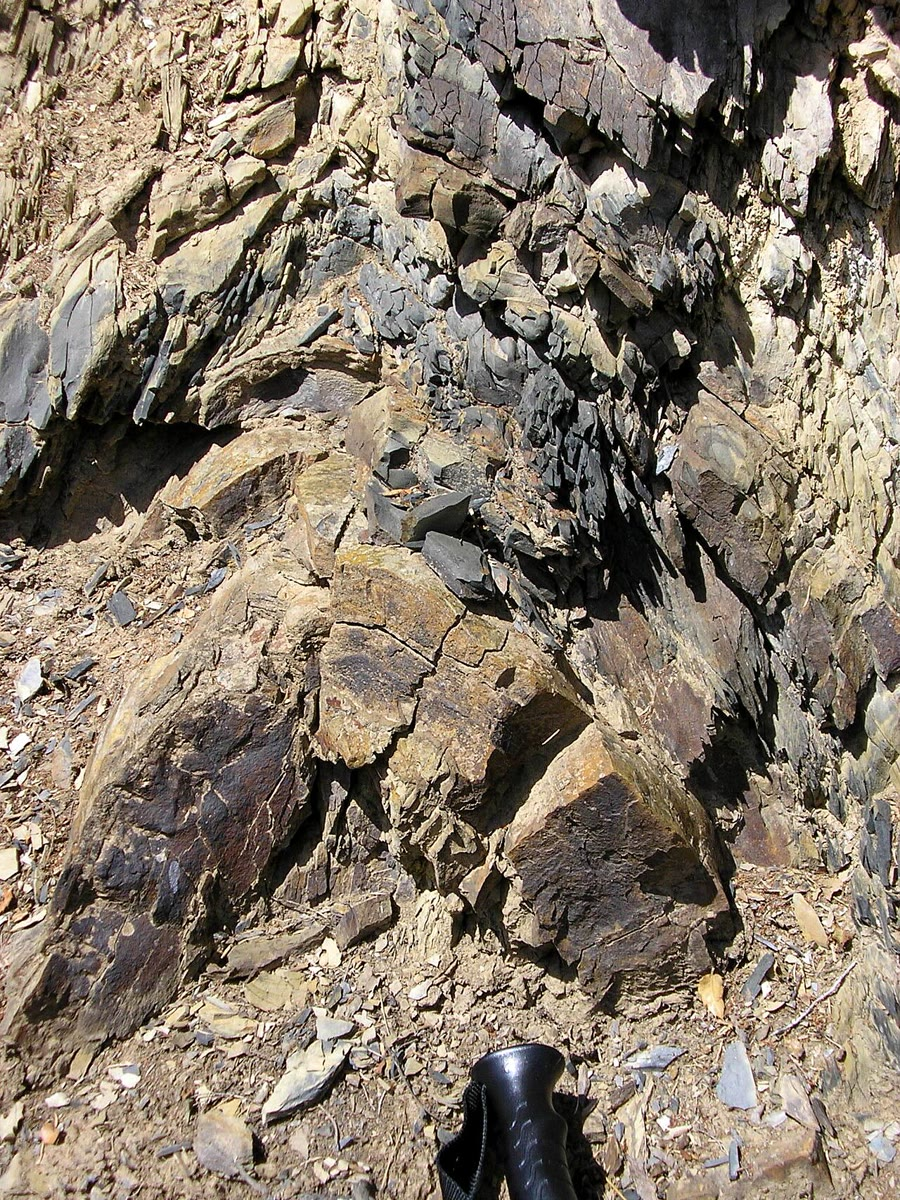
\includegraphics[height=8.2cm]{images/book3/b1-axial-planar-cleavage.jpg}
\par\smallskip{\small 坎塔布里亚的波特斯附近，石炭纪砂岩与页岩互层中的一个小\omterm{def:b1:geological-maps:fold}{背斜}。
图中央下部的褐色砂岩层拱起于\omterm{def:b1:faults-folds-fabrics:fold-elements}{转折端}之上；其上方的深色页岩中，
\omterm{def:b1:faults-folds-fabrics:foliation}{劈理}为一组穿过岩层、陡峭且间距很小的裂隙，
是\omterm{def:b1:faults-folds-fabrics:foliation}{轴面劈理}：它与\omterm{def:b1:geological-maps:fold}{褶皱轴}面近似平行，
并在\omterm{def:b1:faults-folds-fabrics:fold-elements}{轴面}两侧呈扇形展开，扇面随岩层而变化。
手杖把手的直径约 \qty{4}{cm}。
照片：Mikenorton, CC~BY-SA~3.0（维基共享资源）。}
\label{fig:b1:faults-folds-fabrics:cleavage}
\end{omfigure}
% ledger: commons:axial-cleavage

\begin{definition}[线理、交线理、拉伸线理]\label{def:b1:faults-folds-fabrics:lineation}
\emph{线理}\index{线理}是贯穿岩石的线状组构，
以其\omterm{def:b1:field-lab-methods-1:trend-plunge}{倾伏向}和\omterm{def:b1:field-lab-methods-1:trend-plunge}{倾伏角}来度量。
\emph{交线理}\index{交线理}是两个面状组构相互切割所形成的一组直线，
例如层理与\omterm{def:b1:faults-folds-fabrics:foliation}{劈理}之间的交线；
\emph{拉伸线理}\index{拉伸线理}由颗粒或卵石构成，
它们沿最大伸长方向被拉长。
\end{definition}
% ledger: ws:fabrics

\begin{proposition}[褶皱的交线理]\label{prop:b1:faults-folds-fabrics:intersection}
在具有\omterm{def:b1:faults-folds-fabrics:foliation}{轴面劈理}的\omterm{def:b1:faults-folds-fabrics:fold-elements}{圆柱状褶皱}中，
层理与\omterm{def:b1:faults-folds-fabrics:foliation}{劈理}的\omterm{def:b1:faults-folds-fabrics:lineation}{交线理}与\omterm{def:b1:faults-folds-fabrics:fold-elements}{枢纽}平行，
在\omterm{def:b1:geological-maps:fold}{褶皱}各处均如此。
\end{proposition}

\begin{proof}
\omterm{def:b1:faults-folds-fabrics:fold-elements}{圆柱状褶皱}的每个层理面都包含其轴的方向。
\omterm{def:b1:faults-folds-fabrics:fold-elements}{轴面}包含与轴平行的\omterm{def:b1:faults-folds-fabrics:fold-elements}{枢纽}线，
故也包含该方向，每个与之平行的\omterm{def:b1:faults-folds-fabrics:foliation}{劈理}面亦然。
两个不平行的平面若包含同一方向，
则它们沿一条该方向的直线相交。
\end{proof}

该命题是野外地质学家求取过大而无法整体看到的\omterm{def:b1:geological-maps:fold}{褶皱}\omterm{def:b1:field-lab-methods-1:trend-plunge}{倾伏角}的途径：
在任一翼的\omterm{def:b1:geological-maps:geological-map}{露头}上，
\omterm{def:b1:faults-folds-fabrics:foliation}{劈理}切割层理所形成的直线即给出\omterm{def:b1:faults-folds-fabrics:fold-elements}{枢纽}线。层理与\omterm{def:b1:faults-folds-fabrics:foliation}{劈理}
二者合起来还能说明更多：\omterm{def:b1:geological-maps:fold}{褶皱}位于何处，以及岩层的顶底朝向如何。

\begin{definition}[倒向]\label{def:b1:faults-folds-fabrics:vergence}
不对称\omterm{def:b1:geological-maps:fold}{褶皱}的\emph{倒向}\index{倒向}是其上部相对于下部
移动所朝向的水平方向：
即\omterm{def:b1:geological-maps:fold}{褶皱}倒转的方向，或对于\omterm{def:b1:faults-folds-fabrics:fold-classes}{斜歪褶皱}而言，
其倾斜所朝向的方向。
\end{definition}
% ledger: ws:vergence

\begin{proposition}[褶皱两翼上的层理与劈理]\label{prop:b1:faults-folds-fabrics:cleavage-bedding}
考虑一个翼为直线、具有\omterm{def:b1:faults-folds-fabrics:foliation}{轴面劈理}的\omterm{def:b1:geological-maps:fold}{褶皱}，所涉及的岩层
在\omterm{def:b1:geological-maps:fold}{褶皱}前为正立，且两翼均自每个\omterm{def:b1:geological-maps:fold}{背斜}\omterm{def:b1:faults-folds-fabrics:fold-elements}{转折端}向下延伸。
在剖面上看：
\begin{enumerate}[label=(\alph*)]
  \item 在层理与\omterm{def:b1:faults-folds-fabrics:foliation}{劈理}\omterm{def:b1:geological-maps:attitude}{倾向}相同的翼上，
        层理比\omterm{def:b1:faults-folds-fabrics:foliation}{劈理}更陡，当且仅当
        该翼倒转；
  \item 使\omterm{def:b1:faults-folds-fabrics:foliation}{劈理}转到层理上的锐角旋转，
        在\omterm{def:b1:geological-maps:fold}{褶皱}两翼上旋转方向相反；在未倒转的翼上，
        它使\omterm{def:b1:faults-folds-fabrics:foliation}{劈理}顶部水平地朝向该翼顶端的
        \omterm{def:b1:geological-maps:fold}{背斜}\omterm{def:b1:faults-folds-fabrics:fold-elements}{转折端}移动。
\end{enumerate}
\end{proposition}

\begin{proof}
沿\omterm{def:b1:faults-folds-fabrics:fold-elements}{枢纽}方向观察，\omterm{def:b1:faults-folds-fabrics:fold-elements}{轴面}向左倾斜，\omterm{def:b1:geological-maps:attitude}{倾角}为
$\gamma$，$0 < \gamma \le \ang{90}$，角度自
指向右的水平方向起沿逆时针计量。\omterm{def:b1:faults-folds-fabrics:foliation}{劈理}与\omterm{def:b1:faults-folds-fabrics:fold-elements}{轴面}平行，
向上倾斜，\omterm{def:b1:geological-maps:attitude}{倾角}为 $\gamma$。在\omterm{def:b1:geological-maps:fold}{背斜}\omterm{def:b1:faults-folds-fabrics:fold-elements}{转折端}处，两翼向下延伸的方向角分别为
$\ang{180} + \gamma - \iota/2$（翼~1）与
$\ang{180} + \gamma + \iota/2$（翼~2），分居\omterm{def:b1:faults-folds-fabrics:fold-elements}{轴面}两侧，
且 $\iota/2 \le \gamma$，因两翼均向下延伸；\omterm{def:b1:geological-maps:fold}{褶皱}序列中的每个翼，
对于其顶端的\omterm{def:b1:geological-maps:fold}{背斜}而言都是上述二者之一。岩层向外变新，
远离\omterm{def:b1:geological-maps:fold}{背斜}核部，沿翼的法线方向
（该法线指向远离\omterm{def:b1:faults-folds-fabrics:fold-elements}{轴面}的一侧）。

翼~1 向左下方延伸：它向左倾，\omterm{def:b1:geological-maps:attitude}{倾角}为 $\gamma - \iota/2$，
比\omterm{def:b1:faults-folds-fabrics:foliation}{劈理}平缓。其向外法线的方向角为 $\ang{90} + \gamma -
\iota/2$，指向上方，岩层为正立。沿向上方向看，它与水平面的夹角为
$\gamma - \iota/2$，因此使\omterm{def:b1:faults-folds-fabrics:foliation}{劈理}转到层理的锐角旋转
为顺时针，旋转角为 $\iota/2$：\omterm{def:b1:faults-folds-fabrics:foliation}{劈理}顶部向右移动，
即指向\omterm{def:b1:faults-folds-fabrics:fold-elements}{枢纽}所在一侧，因该翼自\omterm{def:b1:faults-folds-fabrics:fold-elements}{枢纽}向左延伸。

翼~2 向上与水平面成 $\gamma + \iota/2$ 的夹角。若
$\gamma + \iota/2 > \ang{90}$，则它向右下方延伸，向右倾，
与\omterm{def:b1:faults-folds-fabrics:foliation}{劈理}\omterm{def:b1:geological-maps:attitude}{倾向}相反；其向外法线的方向角为 $\ang{270} + \gamma +
\iota/2$，向上分量为 $-\cos(\gamma + \iota/2) > 0$：岩层为正立。
若 $\gamma + \iota/2 < \ang{90}$，则它向左下方延伸，
向左倾，\omterm{def:b1:geological-maps:attitude}{倾角}为 $\gamma + \iota/2$，比\omterm{def:b1:faults-folds-fabrics:foliation}{劈理}更陡，
同一分量为负：该翼倒转。两种情形下，使\omterm{def:b1:faults-folds-fabrics:foliation}{劈理}转到层理的锐角旋转
均为逆时针，旋转角为 $\iota/2$，
并使\omterm{def:b1:faults-folds-fabrics:foliation}{劈理}顶部向左移动；当该翼为正立时，
它自\omterm{def:b1:faults-folds-fabrics:fold-elements}{枢纽}向右延伸，故\omterm{def:b1:faults-folds-fabrics:fold-elements}{枢纽}位于左侧。与\omterm{def:b1:faults-folds-fabrics:foliation}{劈理}\omterm{def:b1:geological-maps:attitude}{倾向}相同的翼
因此，\omterm{def:b1:geological-maps:attitude}{倾向}与\omterm{def:b1:faults-folds-fabrics:foliation}{劈理}相同的翼中，较平缓者为翼~1，
较陡且倒转者为翼~2，即为 (a)；翼~1 上为顺时针，
翼~2 上为逆时针，即为 (b)。
\end{proof}

因此，旋转方向在每个\omterm{def:b1:faults-folds-fabrics:fold-elements}{转折端}（无论\omterm{def:b1:geological-maps:fold}{背斜}还是\omterm{def:b1:geological-maps:fold}{向斜}）处都会改变。
地质学家沿一条路线记录这一旋转方向时，便能找到过大而无法
在一个\omterm{def:b1:geological-maps:geological-map}{露头}中看到的\omterm{def:b1:geological-maps:fold}{褶皱}\omterm{def:b1:faults-folds-fabrics:fold-elements}{转折端}（旋转方向改变之处），以及
层理比\omterm{def:b1:faults-folds-fabrics:foliation}{劈理}更陡的倒转翼；“\omterm{def:b1:faults-folds-fabrics:vergence}{倒向}”一词也用于指这种旋转方向，
小\omterm{def:b1:geological-maps:fold}{褶皱}\omterm{def:b1:faults-folds-fabrics:vergence}{倒向}的反转也以同样方式
用于确定大\omterm{def:b1:geological-maps:fold}{褶皱}的\omterm{def:b1:faults-folds-fabrics:fold-elements}{转折端}：一大\omterm{def:b1:geological-maps:fold}{褶皱}两翼上的小\omterm{def:b1:geological-maps:fold}{褶皱}
具有相反的不对称性，大\omterm{def:b1:geological-maps:fold}{褶皱}的轴迹
位于二者之间。
% ledger: ws:vergence, ws:fold-elements

\begin{omfigure}
\begin{tikzpicture}[>={Stealth[length=5pt]}, font=\small]
% a train of chevron folds seen along the hinge (north into the page, east to the right):
% axial planes dipping 60 deg to the west, interlimb angle 40 deg; long limbs dip 40 deg W
% (the right way up), short limbs 80 deg W (overturned). Short limb: from an anticline hinge H_k,
% length s along 260 deg to the syncline hinge S_k; long limb back up along 40 deg to H_{k+1},
% so that all anticline hinges are level, a wavelength w apart.
% Five bedding surfaces, repeated along the axial direction (similar folds); cleavage parallel to it.
\def\s{2.6}
\pgfmathsetmacro{\sx}{\s*cos(260)}\pgfmathsetmacro{\sy}{\s*sin(260)}
\pgfmathsetmacro{\w}{\sx - \sy/tan(40)}
\pgfmathsetmacro{\hx}{0.62*cos(60)}\pgfmathsetmacro{\hy}{0.62*sin(60)}
\newcommand{\surface}[1]{%
  (-\w+#1*\hx, #1*\hy) \foreach \k in {-1,0,1,2,3} { -- ({\k*\w+\sx+#1*\hx}, {\sy+#1*\hy}) -- ({(\k+1)*\w+#1*\hx}, {#1*\hy}) }}
\begin{scope}
  \clip (0.35,-3.3) rectangle (10.0,2.95);
  \begin{scope}
    \clip \surface{0} -- (12,6) -- (-4,6) -- cycle;
    \clip \surface{4} -- (12,-6) -- (-4,-6) -- cycle;
    \fill[omLithSand!45] (-4,-6) rectangle (12,6);
    \fill[omLithShale!40] \surface{2} -- (12,6) -- (-4,6) -- cycle;
    \fill[omLithSand!45] \surface{3} -- (12,6) -- (-4,6) -- cycle;
    \foreach \c in {-8.0,-7.78,...,13.0} {
      \draw[omDef!85, line width=0.35pt] ({\c-6*cot(60)},-6) -- ({\c+6*cot(60)},6);
    }
  \end{scope}
  \foreach \j in {0,1,2,3,4} { \draw[line width=0.75pt, line join=round] \surface{\j}; }
\end{scope}
% axial traces through the anticline hinges, and labels
\foreach \k in {1,2,3} {
  \draw[omThm, dashed, line width=0.6pt] ({\k*\w-0.5*cos(60)},{-0.5*sin(60)}) -- ({\k*\w+3.6*cos(60)},{3.6*sin(60)});
  \node[omThm, font=\scriptsize, anchor=south] at ({\k*\w+3.6*cos(60)},{3.6*sin(60)}) {背斜};
}
\foreach \k in {1,2,3} { \node[omThm, font=\scriptsize, anchor=north] at ({\k*\w+\sx},{\sy-0.15}) {向斜}; }
\end{tikzpicture}
\par\smallskip{\small 一列向右倒转的人字形\omterm{def:b1:geological-maps:fold}{褶皱}，以剖面表示，
带\omterm{def:b1:faults-folds-fabrics:foliation}{轴面劈理}（细蓝线），按比例绘制：\omterm{def:b1:faults-folds-fabrics:fold-elements}{轴面}
向左倾斜 \ang{60}，\omterm{def:b1:faults-folds-fabrics:fold-elements}{翼间角} \ang{40}。长翼
向左倾斜 \ang{40}，比\omterm{def:b1:faults-folds-fabrics:foliation}{劈理}更缓，
且正立；短翼向左倾斜 \ang{80}，比\omterm{def:b1:faults-folds-fabrics:foliation}{劈理}更陡，
且倒转。沿锐角将\omterm{def:b1:faults-folds-fabrics:foliation}{劈理}转到层理上，
其转向在每个长翼上为顺时针，在每个
短翼上为逆时针。\omterm{def:b1:geological-maps:fold}{褶皱}的倾覆方向向右。}
\label{fig:b1:faults-folds-fabrics:vergence}
\end{omfigure}

\section{显微构造}\label{sec:b1:faults-folds-fabrics:micro}

在显微镜下，岩石的变形体现在其颗粒上。一颗
石英颗粒因晶格缓慢滑移而弯曲，在\omterm{def:b1:field-lab-methods-1:microscope}{正交偏光}下不再同时消光：
载物台转动时，一条暗带扫过颗粒，
这是因为颗粒各部分的方向略有不同。
这种波状消光（见\cref{ch:b1:optical-mineralogy}）随着
接近剪切带而增强，因为晶格中的缺陷不断堆积。
有水存在时，颗粒在受压最强的面上溶解，
溶解的物质则在应力较低处沉积，或被带走：
这种压溶作用使岩石在低温下缩短，
并形成许多\omterm{def:b1:faults-folds-fabrics:foliation}{劈理}。温度较高时，受应变的颗粒
在变形持续进行的同时，被新生的、较小的、未受应变的颗粒取代，
首先沿旧颗粒边界发生，即动力重结晶，它使颗粒变小，
并形成\omterm{def:b1:faults-folds-fabrics:fault-rocks}{糜棱岩}。变形颗粒的形状，以及在其影子中生长的\omterm{def:b1:rock-forming-minerals:mineral}{矿物}，
也显示剪切带的运动方向；这些剪切运动指示标志，以及
机制本身，属于本科三年级分册的内容。
% ledger: ws:microstructures, ws:fabrics

\section{练习}

\begin{exercise}[$\star$]\label{exo:b1:faults-folds-fabrics:1}
根据各断层\omterm{def:b1:faults-folds-fabrics:fault-elements}{滑动矢量}的\omterm{def:b1:faults-folds-fabrics:fault-elements}{侧伏角}命名断层，断层面\omterm{def:b1:geological-maps:attitude}{倾角}为 \ang{60}：
(a) $r = \ang{-90}$；(b) $r = \ang{85}$；(c) $r = 0$；(d) $r = \ang{180}$；
(e) $r = \ang{-40}$。(f) 若 (b) 中的\omterm{def:b1:geological-maps:attitude}{倾角}为 \ang{25}，则该断层应称为何种断层？
% ledger: ar:rake, usgs:fault-types
\end{exercise}

\begin{exercise}[$\star$]\label{exo:b1:faults-folds-fabrics:2}
\omterm{def:b1:faults-folds-fabrics:fault-types}{正断层}的\omterm{def:b1:geological-maps:attitude}{倾角}为 \ang{55}，其滑动为纯倾滑，\omterm{def:b1:faults-folds-fabrics:fault-elements}{总滑距}为
\qty{300}{m}。求其\omterm{def:b1:cross-sections:throw}{垂直断距}和\omterm{def:b1:cross-sections:throw}{水平断距}。
\end{exercise}

\begin{exercise}[$\star$]\label{exo:b1:faults-folds-fabrics:3}
求各\omterm{def:b1:faults-folds-fabrics:fold-classes}{直立褶皱}的\omterm{def:b1:faults-folds-fabrics:fold-elements}{翼间角}及其类型，两翼\omterm{def:b1:geological-maps:attitude}{倾向}相反，\omterm{def:b1:geological-maps:attitude}{倾角}分别为：
(a) 两翼\omterm{def:b1:geological-maps:attitude}{倾角}均为 \ang{35}；(b) \ang{70}
与 \ang{75}；(c) \ang{85} 与 \ang{88}。
% ledger: ws:fold-classes
\end{exercise}

\begin{exercise}[$\star$]\label{exo:b1:faults-folds-fabrics:4}
某砂岩的\omterm{def:b1:stress-strain-rheology:coulomb}{内摩擦角}为 \ang{35}。依据安德森理论，
求其\omterm{def:b1:faults-folds-fabrics:fault-types}{正断层}与\omterm{def:b1:faults-folds-fabrics:fault-types}{逆冲断层}的\omterm{def:b1:geological-maps:attitude}{倾角}各为多少？
两条共轭\omterm{def:b1:faults-folds-fabrics:fault-types}{走滑断层}之间的夹角为多少？
\end{exercise}

\begin{exercise}[$\star\star$]\label{exo:b1:faults-folds-fabrics:5}
某断层的\omterm{def:b1:geological-maps:attitude}{产状}为 $090/50$，其断层面上\omterm{def:b1:faults-folds-fabrics:fault-rocks}{擦痕}的\omterm{def:b1:faults-folds-fabrics:fault-elements}{侧伏角}为 \ang{-30}；
\omterm{def:b1:faults-folds-fabrics:fault-elements}{总滑距}为 \qty{400}{m}。(a) 求走滑分量和倾滑分量，
以及\omterm{def:b1:cross-sections:throw}{垂直断距}和\omterm{def:b1:cross-sections:throw}{水平断距}。(b) 以东、北、上分量写出\omterm{def:b1:faults-folds-fabrics:fault-elements}{滑动矢量}，
并给出其\omterm{def:b1:field-lab-methods-1:trend-plunge}{倾伏向}和\omterm{def:b1:field-lab-methods-1:trend-plunge}{倾伏角}。(c) 为该断层命名。
\end{exercise}

\begin{exercise}[$\star\star$]\label{exo:b1:faults-folds-fabrics:6}
两条同期的直立\omterm{def:b1:faults-folds-fabrics:fault-types}{走滑断层}，\omterm{def:b1:geological-maps:attitude}{走向}分别为 $020$ 和 $080$。
(a) 依据安德森理论，给出 $\sigma_1$、$\sigma_2$ 和
$\sigma_3$ 的方向，以及岩石的\omterm{def:b1:stress-strain-rheology:coulomb}{内摩擦角}。(b) 哪条断层是\omterm{def:b1:faults-folds-fabrics:fault-types}{右行}的，
哪条是\omterm{def:b1:faults-folds-fabrics:fault-types}{左行}的？请依据沿 $\sigma_1$ 方向的缩短加以论证。
\end{exercise}

\begin{exercise}[$\star\star$]\label{exo:b1:faults-folds-fabrics:7}
\omterm{def:b1:faults-folds-fabrics:fold-elements}{圆柱状褶皱}的两翼\omterm{def:b1:geological-maps:attitude}{产状}分别为 $120/40$ 和 $260/30$。
利用\cref{prop:b1:faults-folds-fabrics:hinge}，求其\omterm{def:b1:faults-folds-fabrics:fold-elements}{枢纽}的\omterm{def:b1:field-lab-methods-1:trend-plunge}{倾伏向}和\omterm{def:b1:field-lab-methods-1:trend-plunge}{倾伏角}，
以及\omterm{def:b1:faults-folds-fabrics:fold-elements}{翼间角}和类型。
\end{exercise}

\begin{exercise}[$\star\star$]\label{exo:b1:faults-folds-fabrics:8}
在一处\omterm{def:b1:geological-maps:geological-map}{露头}，层理的\omterm{def:b1:geological-maps:attitude}{产状}为 $040/30$，\omterm{def:b1:faults-folds-fabrics:foliation}{轴面
劈理}的\omterm{def:b1:geological-maps:attitude}{产状}为 $160/80$。求\omterm{def:b1:faults-folds-fabrics:lineation}{交线理}的\omterm{def:b1:field-lab-methods-1:trend-plunge}{倾伏向}和\omterm{def:b1:field-lab-methods-1:trend-plunge}{倾伏角}。
这对该\omterm{def:b1:geological-maps:fold}{褶皱}说明了什么？
\end{exercise}

\begin{exercise}[$\star\star$]\label{exo:b1:faults-folds-fabrics:9}
一条直立断层\omterm{def:b1:geological-maps:attitude}{走向}为东西向，一条\omterm{def:b1:geological-maps:attitude}{走向}为南北向的直立岩墙
与之相交；断层以北的岩墙位于其在断层以南位置以东 \qty{350}{m}
处。(a) 该断层是\omterm{def:b1:faults-folds-fabrics:fault-types}{右行}还是\omterm{def:b1:faults-folds-fabrics:fault-types}{左行}？(b) 若\omterm{def:b1:faults-folds-fabrics:fault-rocks}{擦痕}水平，
则\omterm{def:b1:faults-folds-fabrics:fault-elements}{总滑距}为多少？(c) 若\omterm{def:b1:faults-folds-fabrics:fault-rocks}{擦痕}改为向东倾伏
\ang{20}，则\omterm{def:b1:faults-folds-fabrics:fault-elements}{总滑距}与滑动的竖直分量各为多少，
以及哪一盘下降？
\end{exercise}

\begin{exercise}[$\star\star\star$]\label{exo:b1:faults-folds-fabrics:10}
设一条\omterm{def:b1:stress-strain-rheology:coulomb}{内聚力}为零、摩擦系数为 $\mu$ 的断层，其夹角 $\theta$
为断层面与 $\sigma_1$ 之间的夹角。(a) 证明：当有效\omterm{def:b1:stress-strain-rheology:principal}{主应力}
之比达到下式所给的值：
\[
  \frac{\sigma_1'}{\sigma_3'} = \frac{1 + \mu\cot\theta}{1 - \mu\tan\theta} .
\]
(b) 取 $\mu = 0.6$，$\sigma_1$ 竖直，计算\omterm{def:b1:faults-folds-fabrics:fault-types}{正断层}在
\omterm{def:b1:geological-maps:attitude}{倾角}分别为 \ang{60}、\ang{45} 和 \ang{35} 时的比值。(c) 证明：\omterm{def:b1:geological-maps:attitude}{倾角}小于某一角度的
\omterm{def:b1:faults-folds-fabrics:fault-types}{正断层}永远不会滑动，并求出该角度。
(d) 对 $\mu = 0.6$ 和 $\mu = 0.85$，给出最优取向的
\omterm{def:b1:faults-folds-fabrics:fault-types}{正断层}和\omterm{def:b1:faults-folds-fabrics:fault-types}{逆冲断层}的\omterm{def:b1:geological-maps:attitude}{倾角}。
\end{exercise}

\begin{exercise}[$\star\star\star$]\label{exo:b1:faults-folds-fabrics:11}
沿一条东西向穿越人字形\omterm{def:b1:geological-maps:fold}{褶皱}的剖面，\omterm{def:b1:geological-maps:fold}{褶皱}\omterm{def:b1:faults-folds-fabrics:fold-elements}{枢纽}\omterm{def:b1:geological-maps:attitude}{走向}为北向，
\omterm{def:b1:faults-folds-fabrics:foliation}{轴面劈理}处处向西倾，\omterm{def:b1:geological-maps:attitude}{倾角}为 \ang{60}。层理
在测站 A、B 和 C 处，层理向西倾，\omterm{def:b1:geological-maps:attitude}{倾角}分别为 \ang{40}、\ang{80} 和 \ang{40}，
测站自西向东排列，岩层在
\omterm{def:b1:geological-maps:fold}{褶皱}前为正常层序。(a) 哪一个测站位于倒转翼上？(b) 在各测站，
面朝北看去，\omterm{def:b1:faults-folds-fabrics:foliation}{劈理}以何种方向转到层理上？
(c) \omterm{def:b1:faults-folds-fabrics:fold-elements}{枢纽}位于何处，哪些为\omterm{def:b1:geological-maps:fold}{背斜}？(d) 求\omterm{def:b1:faults-folds-fabrics:fold-elements}{翼间角}
及\omterm{def:b1:faults-folds-fabrics:fold-elements}{轴面}\omterm{def:b1:geological-maps:attitude}{产状}，并说明这些\omterm{def:b1:geological-maps:fold}{褶皱}的
\omterm{def:b1:faults-folds-fabrics:vergence}{倒向}。
\end{exercise}

\begin{exercise}[$\star\star\star$]\label{exo:b1:faults-folds-fabrics:12}
一层长度为 $L_0$ 的岩层，被折叠成一组对称人字形\omterm{def:b1:geological-maps:fold}{褶皱}，
其\omterm{def:b1:faults-folds-fabrics:fold-elements}{翼间角}为 $\iota$，长度保持不变。(a) 证明：其
横向测得的长度变为 $L_0\sin(\iota/2)$。(b) \omterm{def:b1:faults-folds-fabrics:fold-elements}{翼间角}为
\ang{60} 的人字形\omterm{def:b1:geological-maps:fold}{褶皱}代表多大的缩短量？(c) 与
\qty{30}{\percent} 缩短量对应的\omterm{def:b1:faults-folds-fabrics:fold-elements}{翼间角}为多少？(d) 一组\omterm{def:b1:faults-folds-fabrics:fold-classes}{直立
褶皱}的翼部\omterm{def:b1:geological-maps:attitude}{倾角}为 \ang{12}，求其缩短量。
\end{exercise}

\section{问题：瓦尔登丘陵的构造测量}

\begin{problem}[{周末问题——瓦尔登丘陵的背斜与正断层，
由其平面产状推算
断层上的滑动}]
\label{pb:b1:faults-folds-fabrics:1}
% values: calc/ch17.py; region: figdata/shared/region.py (limbs, plunge, fault)
瓦尔登丘陵被\omterm{def:b1:geological-maps:fold}{褶皱}成一个\omterm{def:b1:geological-maps:fold}{背斜}，其轴向为南北向，
位于 $x = \qty{3.5}{km}$ 处，东侧 \qty{4}{km} 处为一个\omterm{def:b1:geological-maps:fold}{向斜}；两者
翼面均为平面。野外调查测得\omterm{def:b1:geological-maps:fold}{背斜}东翼的层理\omterm{def:b1:geological-maps:attitude}{产状}为
$080.7/12.2$，西翼为 $279.3/12.2$。覆盖层
被一条\omterm{def:b1:geological-maps:attitude}{产状}为 $120/60$ 的\omterm{def:b1:faults-folds-fabrics:fault-types}{正断层}切割，其\omterm{def:b1:faults-folds-fabrics:fault-elements}{上盘}沿\omterm{def:b1:geological-maps:attitude}{倾向}下滑，
\omterm{def:b1:cross-sections:throw}{垂直断距}为 \qty{200}{m}。角度精确到 \ang{0.1}，长度精确到
\qty{0.1}{m}。

\medskip
\noindent\textbf{第一部分——两翼。}
\begin{enumerate}
  \item 写出向上的单位法向量 $\mathbf n_1$（东翼）和
        $\mathbf n_2$（西翼），用东、北、上分量表示。
  \item 计算 $\mathbf n_1\cdot\mathbf n_2$ 及
        两法向量之间的夹角。
  \item 由此推出\omterm{def:b1:geological-maps:fold}{背斜}的\omterm{def:b1:faults-folds-fabrics:fold-elements}{翼间角}。
  \item 依据\omterm{def:b1:faults-folds-fabrics:fold-elements}{翼间角}对该\omterm{def:b1:geological-maps:fold}{背斜}进行分类。
  \item 两翼的\omterm{def:b1:geological-maps:attitude}{倾角}均为 \ang{12.2}。为何\omterm{def:b1:faults-folds-fabrics:fold-elements}{翼间角}不恰好等于
        $\ang{180} - 2\times\ang{12.2}$？计算任一翼在
        东西向竖直剖面中的\omterm{def:b1:cross-sections:apparent-dip}{视倾角}。
  \item \omterm{def:b1:geological-maps:fold}{向斜}与\omterm{def:b1:geological-maps:fold}{背斜}共用东翼，其自身的东翼
        与\omterm{def:b1:geological-maps:fold}{背斜}的西翼平行。求该\omterm{def:b1:geological-maps:fold}{向斜}的
        \omterm{def:b1:faults-folds-fabrics:fold-elements}{翼间角}。
\end{enumerate}

\medskip
\noindent\textbf{第二部分——\omterm{def:b1:faults-folds-fabrics:fold-elements}{枢纽}线与\omterm{def:b1:faults-folds-fabrics:fold-elements}{轴面}。}
\begin{enumerate}[resume]
  \item 计算 $\mathbf n_1\times\mathbf n_2$，并求
        \omterm{def:b1:faults-folds-fabrics:fold-elements}{枢纽}线的\omterm{def:b1:field-lab-methods-1:trend-plunge}{倾伏向}和\omterm{def:b1:field-lab-methods-1:trend-plunge}{倾伏角}。
  \item 给出\omterm{def:b1:faults-folds-fabrics:fold-elements}{轴面}的\omterm{def:b1:geological-maps:attitude}{产状}。该\omterm{def:b1:geological-maps:fold}{背斜}是直立的、
        斜歪的还是平卧的？
  \item 给出该\omterm{def:b1:geological-maps:fold}{褶皱}的完整描述：紧闭程度、
        \omterm{def:b1:faults-folds-fabrics:fold-elements}{轴面}\omterm{def:b1:geological-maps:attitude}{产状}及\omterm{def:b1:field-lab-methods-1:trend-plunge}{倾伏角}。
  \item 在\cref{ch:b1:geological-maps}的\omterm{def:b1:geological-maps:geological-map}{地质图}上，\omterm{def:b1:geological-maps:fold}{背斜}的\omterm{def:b1:geological-maps:geological-map}{露头}
        朝哪个方向闭合，其核部出露的是什么？
  \item 覆盖层中的页岩发育\omterm{def:b1:faults-folds-fabrics:foliation}{轴面劈理}。给出其
        \omterm{def:b1:geological-maps:attitude}{产状}，并求其在东翼上的\omterm{def:b1:faults-folds-fabrics:lineation}{交线理}的\omterm{def:b1:field-lab-methods-1:trend-plunge}{倾伏向}
        及\omterm{def:b1:field-lab-methods-1:trend-plunge}{倾伏角}。
  \item 在东翼上，面朝北看去，\omterm{def:b1:faults-folds-fabrics:foliation}{劈理}以何种方向转向
        层理，且\omterm{def:b1:geological-maps:fold}{背斜}\omterm{def:b1:faults-folds-fabrics:fold-elements}{枢纽}位于哪一侧？
\end{enumerate}

\medskip
\noindent\textbf{第三部分——断层与应力。}
\begin{enumerate}[resume]
  \item 按右手法则给出断层的\omterm{def:b1:geological-maps:attitude}{走向}，并说明
        \omterm{def:b1:faults-folds-fabrics:fault-elements}{上盘}位于其迹线的哪一侧。
  \item 依据安德森理论，断层形成时竖直方向的是
        哪一个\omterm{def:b1:stress-strain-rheology:principal}{主应力}？
  \item 给出两个水平\omterm{def:b1:stress-strain-rheology:principal}{主应力}的方向。
  \item \omterm{def:b1:geological-maps:attitude}{倾角}意味着多大的\omterm{def:b1:stress-strain-rheology:coulomb}{内摩擦角}？\omterm{def:b1:stress-strain-rheology:coulomb}{内摩擦系数}
        为多少？
  \item 给出同一应力场可能形成的共轭断层组的\omterm{def:b1:geological-maps:attitude}{产状}，
        以及两组断层之间的夹角。
  \item 在同一应力状态下，该断层是否仍最有利于滑动，
        按\omterm{prop:b1:stress-strain-rheology:byerlee}{拜尔利定律}取摩擦系数 0.85？
\end{enumerate}

\medskip
\noindent\textbf{第四部分——滑动。}
\begin{enumerate}[resume]
  \item 给出\omterm{def:b1:faults-folds-fabrics:fault-elements}{滑动矢量}的\omterm{def:b1:faults-folds-fabrics:fault-elements}{侧伏角}，以及其\omterm{def:b1:field-lab-methods-1:trend-plunge}{倾伏向}和\omterm{def:b1:field-lab-methods-1:trend-plunge}{倾伏角}。
  \item 用东、北、上分量写出滑动的单位矢量。
  \item 计算断层的\omterm{def:b1:cross-sections:throw}{水平断距}。
  \item 计算\omterm{def:b1:faults-folds-fabrics:fault-elements}{上盘}水平位移的东向
        和北向分量。
  \item 验证\omterm{def:b1:faults-folds-fabrics:fault-elements}{总滑距} $L$、\omterm{def:b1:cross-sections:throw}{垂直断距} $h$ 和\omterm{def:b1:cross-sections:throw}{水平断距} $e$ 满足
        $L^2 = h^2 + e^2$，并说明其原因。
  \item 精确到米，瓦尔登断层的\omterm{def:b1:faults-folds-fabrics:fault-elements}{总滑距}为多少？
\end{enumerate}
\end{problem}
